\chapter{STUDY I - FOOT DETECTION AND PRIMARY DIAGNOSIS}\label{chp:Foot Detection & Primary Diagnosis}

This chapter provides an overview of the primary system. Unlike other example solutions, the proposed approach will contain progressive updates with collected data over time. That is why the initial study contains fundamental structures to conduct the research. Accordingly, in Section \ref{sec:StudyIAnalysisAndDesign}, discusses general system analysis and design decisions. Section \ref{sec:StudyIImplementation} covers detailed implementation of the prototype system, and lastly, Section \ref{sec:StudyITestAndEvaluation} presents evaluation phase and initial test results.

\section{ANALYSIS AND DESIGN}\label{sec:StudyIAnalysisAndDesign}

The system, when used by patients, calculates a preliminary detection of potential pes planus and pes cavus. Therefore, end-user interface, healthcare interface, back-end services, and database are needed. Each structure contains its own development life-cycle to provide the best results. The proposed structure of the system can be seen in Figure \ref{fig:GeneralArchitectureDiagram}.

\begin{figure}[htbp]
\centering
\fbox{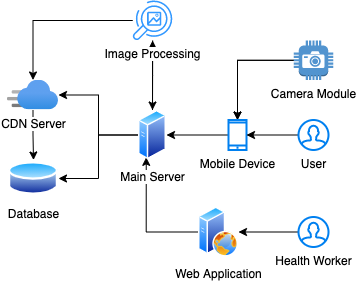
\includegraphics[width=.6\columnwidth]{figures/GeneralArchitectureDiagram.png}}
\caption{Architecture diagram}
\label{fig:GeneralArchitectureDiagram}
\end{figure}

The goal of the study is to assist the medical staff in detecting pes planus and pes cavus and reduce the workload of medical staff. The system to be formed at the end of the study should provide basic functional requirements and as well as non-functional requirements, which are detailed below;
\begin{itemize}
  \item Detection of pes planus and pes cavus with at most accuracy in provided images.
  \item Detects predefined extreme health cases and redirects users to healthcare professionals.
  \item Verify the results manually with an interface for experts
  \item View detection results
  \item Provide statistical reports about pes planus and pes cavus
  \item Provide the functionality to a wide range of users on multiple mobile platforms.
  \item Store all confidential information securely
  \item Store all essential information in non-volatile storage
  \item Design scalable system for large scale usage
\end{itemize}

\begin{figure}[htbp]
\centering
\fbox{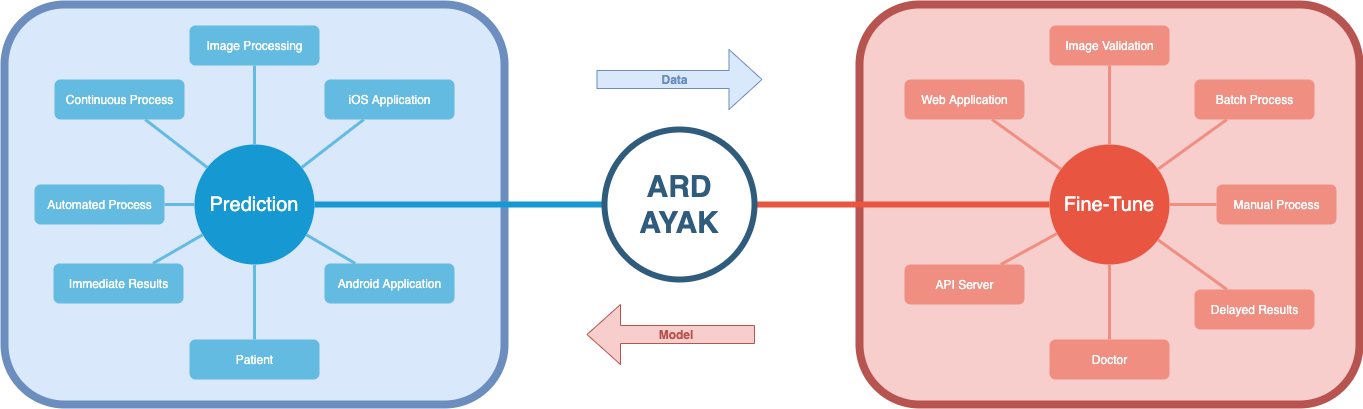
\includegraphics[width=.9\columnwidth]{figures/PredictionAndFinetuneModules.png}}
\caption{Prediction and fine-tune modules}
\label{fig:PredictionAndFinetuneModules}
\end{figure}

Furthermore, all the services should not be accessible by unauthorized users since the system contains confidential information. Therefore, the same authorization process should be used in all information access. In addition, for research purposes, user data will be purified from user-identifying information when calculating measurement methods imposed by KVKK and GDPR, such as phone numbers.

The system should contain two essential components in order to provide a stable service: the prediction and fine-tune modules. In addition, modules should support each other and improve the process, as shown in Figure \ref{fig:PredictionAndFinetuneModules}.

\subsection{ Prediction Module }

The prediction module should essentially consist of two parts, namely end-user and pre-diagnosis algorithms. The end-user application will provide remote access, which is one of the priorities of the system, to the user. Thus, patients will be provided with healthcare services without going to the hospital. To this end, mobile applications should provide services to 95 percent of the mobile operating systems in the market, which are mainly made of iOS and Android operating systems. After user information is collected through the end-user application, pre-diagnosis algorithms will be used to diagnose the user and provide results.

In the prediction module, user information collection is one of the fundamental parts. Information collection should be divided into three fundamental headings: essential, health, and foot information. 

The essential information collection part focuses on differentiating end-users. Therefore, unique properties such as users' phone numbers or email addresses should be collected as part of this heading. Furthermore, gender, birth date, weight, and height should also be collected to analyze the population variance. Even if it is not related, the terms and conditions document that asks the user to confirm data usage and storage permission also should be viewed and agreed upon under this heading.

The second part is the health information collection which focus on detecting health issues related to pes planus and pes cavus. However, this part also requires the system to detect the evaluation requirement of health professionals for critical health issues. Therefore, the system should propose a direct call or appointment for the face-to-face examination between the user and health professional in such conditions. Furthermore, discovering critical health issues should be based on a rule-based system to reduce errors. However this is expected to be very limited to specified cases such as extreme pain levels.

Finally, the foot information collection part should focus on detecting pes planus and pes cavus. Therefore, the degree of pain in physical activities, the degree of pain at night, and most importantly, pictures of the foot should be collected. In Figure \ref{fig:PredictionModuleSequenceDiagram}, the sequence diagram of the prediction module can be seen.

\begin{figure}[htbp]
\centering
\fbox{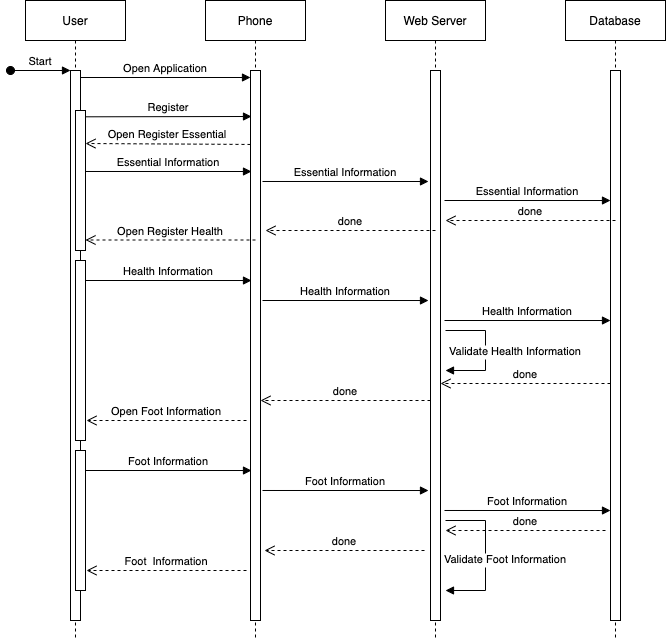
\includegraphics[width=.9\columnwidth]{KaanEksenMSc/figures/PredictionModuleSequenceDiagram.png}}
\caption{Prediction module sequence diagram}
\label{fig:PredictionModuleSequenceDiagram}
\end{figure}

In the prediction module, the collected information should also inform health professionals in order to reduce examination time. Besides that, in Section \ref{sec:FineTuneModule}, Fine Tune Module, the system performance improvement step, which is formed by adding new data to be obtained from health professionals, will be discussed.

In addition, all end-user applications should be user-friendly and provide sufficient feedback information for users. This feedback will improve user satisfaction and reduce the overall process's time consumption, such as application usage instructions.

Last but not least, the prediction module collects statistical data as part of the survey. Conducting surveys through the end-user applications will allow the system to reduce UI shortcomings. Apart from these, the same surveys will also enable healthcare professionals to receive feedback on actively performed healing procedures. Some procedures require users to perform actions on a daily or weekly basis. Therefore surveying these actions to improve users' overall experience on digital healthcare is of utmost importance for the system to be more user friendly.

\subsection{ Fine-Tune Module }\label{sec:FineTuneModule}

The fine-tuning module, which is the central part, should include background procedures and healthcare professionals' interface. In order to achieve this, the module should implement two functionality namely system enhancement and user interface. Accordingly, in order to provide workflow, healthcare professionals, also known as system managers, should review and analyze user-provided data, which should be used to refine system diagnoses process. Eventually, the system should actively enhance the pre-diagnosis process by using the data doctored and adjusted by the system managers.

\begin{figure}[htbp]
\centering
\fbox{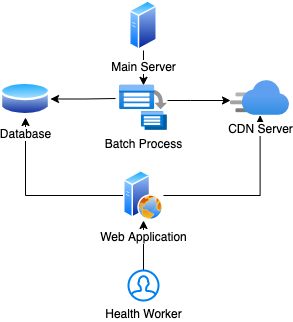
\includegraphics[width=.5\columnwidth]{figures/FineTuneModuleDiagram.png}}
\caption{Fine-tune module diagram}
\label{fig:FineTuneModuleDiagram}
\end{figure}

As can be seen in Figure \ref{fig:FineTuneModuleDiagram}, a web application should be implemented for system managers to display and review the user input, such as foot images, previous diseases. In the web application, system managers should be able to calculate foot types with objective measurement methods such as the Staheli arch index with provided images from the user. As a result of this calculation, there will be two results, one provided from the doctor, and one generated by the system which can be later compared.


System managers supply data in an orderly fashion in dual circles; provide, validate (see Figure \ref{fig:FineTuneModuleWebApplicationActivityDiagram}). Healthcare professionals view patient information in the provided cycle and contribute foot type detection inputs. Information viewing involves primary data (BMI, Shoe Size), patient complaints (pain level, pain duration), health history (surgeries and chronic diseases), and foot pictures. Afterward, foot type detection inputs are provided by health workers. As a result of detection inputs, the system should be able to calculate multiple foot indexes. In Figure \ref{fig:FineTuneModuleWebApplicationSequenceDiagram}, the sequence diagram of the fine-tune module can be seen.

\begin{figure}[htbp]
\centering
\fbox{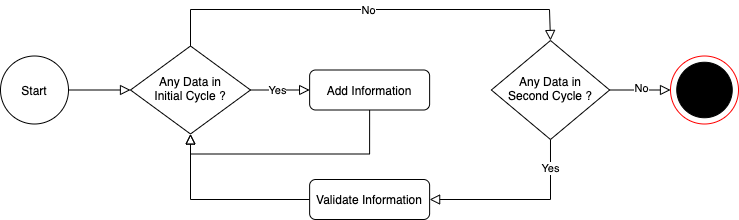
\includegraphics[width=.8\columnwidth]{figures/FineTuneModuleWebApplicationActivityDiagram.png}}
\caption{Fine-Tune Module - Web Application - Activity Diagram}
\label{fig:FineTuneModuleWebApplicationActivityDiagram}
\end{figure}

At the end of the initial cycle, the system should calculate well known accepted foot indexes using key points obtained from healthcare professionals. These indexes should be pre-defined such as Chippaux-Smirak Index, Arch Height Index.

\begin{figure}[htbp]
\centering
\fbox{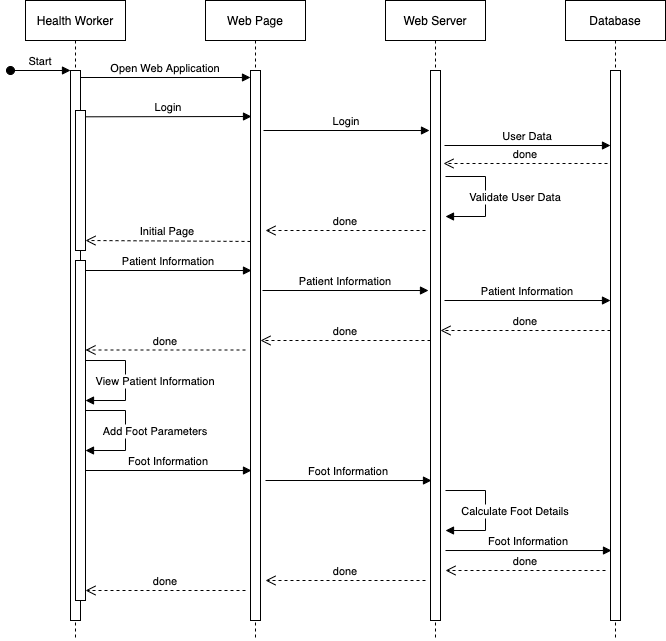
\includegraphics[width=.9\columnwidth]{figures/FineTuneModuleWebApplicationSequenceDiagram.png}}
\caption{Fine-tune module web application activity diagram}
\label{fig:FineTuneModuleWebApplicationSequenceDiagram}
\end{figure}

The second cycle should provide the calculated data to healthcare officials to validate the results. The system user should see how the results are calculated, related user data, and other meaningful information in this second cycle. At this stage healthcare professionals can respond to each of the results as move to initial cycle, unusable or approved. Accordingly, the approved results should be used to improve batch process performance

Furthermore, the second cycle should also focus on preventing any user-related errors. Therefore, multiple calculation results, formulas, and corresponding result statuses (pes planus and pes cavus) should be displayed to reduce the errors. In addition, the system should be able to rewind the cycle to the initial state is based on healthcare professionals' decisions.

\subsection{ Batch Process }

The batch process should be designed to improve the pre-diagnosis with the data provided from the prediction and fine-tune module. Besides being able to trigger manually, the batch process should be automated for continuous learning. Therefore, this will provide the system to improve itself over time through the data provided by the modules (doctors and patients). 

\begin{figure}[htbp]
\centering
\fbox{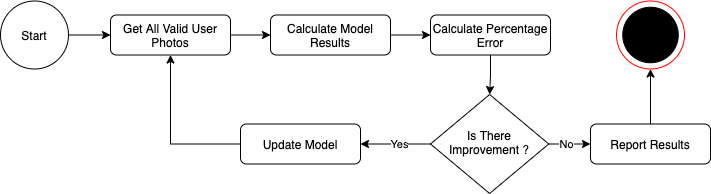
\includegraphics[width=.9\columnwidth]{figures/BatchProcessActivityDiagram.png}}
\caption{Batch process activity diagram}
\label{fig:BatchProcessActivityDiagram}
\end{figure}

The batch process should consist of four basic steps. Firstly, the batch process should get all the valid user-provided photos from the prediction module. Then, the system should process all the images on the current model and calculate the results. After the calculation, the batch process should calculate percentage errors with provided data from healthcare professionals. Then, based on results and improvement strategy, the model is updated or not. Finally, all the calculations should be redone when the model is updated until the best results are obtained. In Figure \ref{fig:BatchProcessActivityDiagram}, the activity diagram of the batch process can be seen.

In addition, the batch process should provide reports about the system's detailed and overview progress, which contains calculated multiple errors. The overview results are a comparison of patients' diagnoses. As a result, this error calculation should provide how successful the system is as a product. Moreover, the detailed error results should be used to improve the system in short cycles. The detailed error calculation should use sub-findings of the system and the calculation points provided by health workers, such as points on the pictures used to identify foot structure. 

\subsection{ Foot Index Calculations }

The system should use multiple methods to find the best approach and assist healthcare professionals in diagnosing patients successfully. Therefore, a fine-tune module system should provide foot indexes, calculation methods used in the examination such as Arch Height Index, Chippaux-Smirak Index, Staheli Index, Clarkes Angle Calculation, Rearfoot Angle Calculation. 

Each calculation type requires its specialty to diagnose accurately, such as the calculation of specific angles of the foot structure. Therefore, the system focuses on a specific type of index calculation, the Arch Height Index, in an automated process to reduce errors.

The arch height index should be calculated using a single foot image. Thus single image usage reduces user workload and improves user experience. In addition, the arch height index requires an image of the foot containing the side of the foot to calculate the index type correctly. This image should be used to detect reference points on the side of the foot. 

Other index calculations are not used for the automated process. They were used only with the data provided by healthcare professionals, which details are explained in the offline phase part. Instead, other index methods are used as reference methods for our calculations. This will allow us to compare different types of measurements. Consequently, the best method for the mobile approach will be selected. The calculation details can be seen in Chapter \ref{chp:Methodology}.

\section{IMPLEMENTATION}\label{sec:StudyIImplementation}

This section discusses the implementation details and decisions of the study. The study contains multiple applications. Each application is divided into its implementation section. In addition, this section starts with the development process subsection, which explains applied development processes for each application.

\subsection{Development Process}

Software engineering is one of the fastest-growing fields in computer science. Over the years, it has had some milestones in development processes. However, in general, iterative development in its core has never changed. The most significant difference in software development processes is the reaction to changes in requirements. Therefore, we applied a hybrid model in our software development processes which are different in each application. This section will provide information regarding this decision and the reasons for it.

Client applications follow the prototype development process since collecting the data was crucial at the start of the development process. In addition, client applications contain dynamic composition where requirements change based on feedback. For example, only the iOS operating system was supported at the beginning of the project, but the Android prototype was also introduced due to the diverse mobile market and the users' need for android applications.

On the other hand, batch processes, which used by the other application in Study I, were less prone to change and had no different types. Therefore, the waterfall development process is adopted. In addition, the server APIs for rapid response to client application changes have continuously improved throughout its lifetime as it fundamentally embraces Agile development.

\subsection{End-User Application}

The end-user system contains two distinct clients, which are iOS and Android. Client applications developed in mind usability, accessibility, inclusion, updated and improved during the application lifecycle. Consequently, this will improve the user experience and be satisfactory for all user groups.

The iOS client is compatible with iOS 11 and forward, making it accessible for 99,7 percent of the market share. Furthermore, mainly Swift programming language is used for the development of the client. Therefore, this makes it easy to support feature updates and compatibility for all the iOS ecosystems. 

\begin{figure}[htbp]
\centering
\fbox{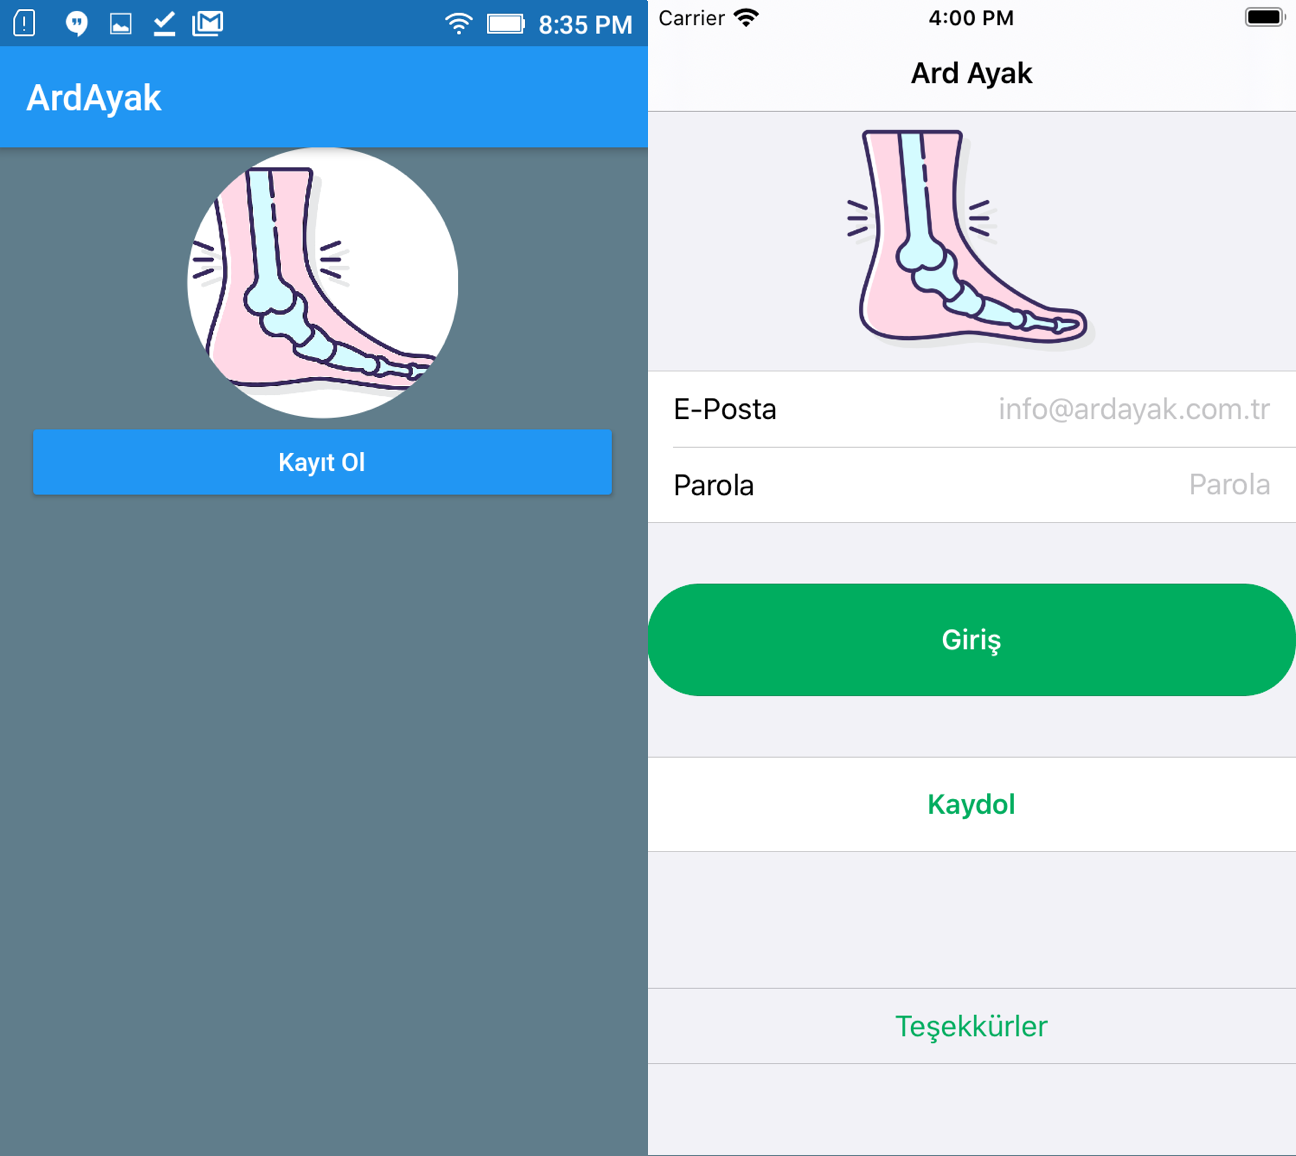
\includegraphics[width=.7\columnwidth]{figures/UserApplicationUI.png}}
\caption{Android (left) and iOS (right) application UI}
\label{fig:UserApplicationUI}
\end{figure}

The android client is compatible with API level 16 and forward, making it accessible for 99,8 percent of the market share. Furthermore, the Flutter software development kit is used in the development process, which requires Dart programming language. Therefore, this makes the software compatible with iOS and Android publishing. On the other hand, the Flutter application is only used for android clients as this process requires additional development. However, this feature can also be used in the future development process to reduce development costs.

Both end-user applications use the same user flow with corresponding platform UI specifications. Therefore this will enable users to complete their operations more comfortably with the UI they frequently use, shown in Figure \ref{fig:UserApplicationUI}. Furthermore, user documentation is also created to help smooth the user experience. This document contains all the information, from how to use it to the download links of the application. 

\begin{figure}[htbp]
\centering
\fbox{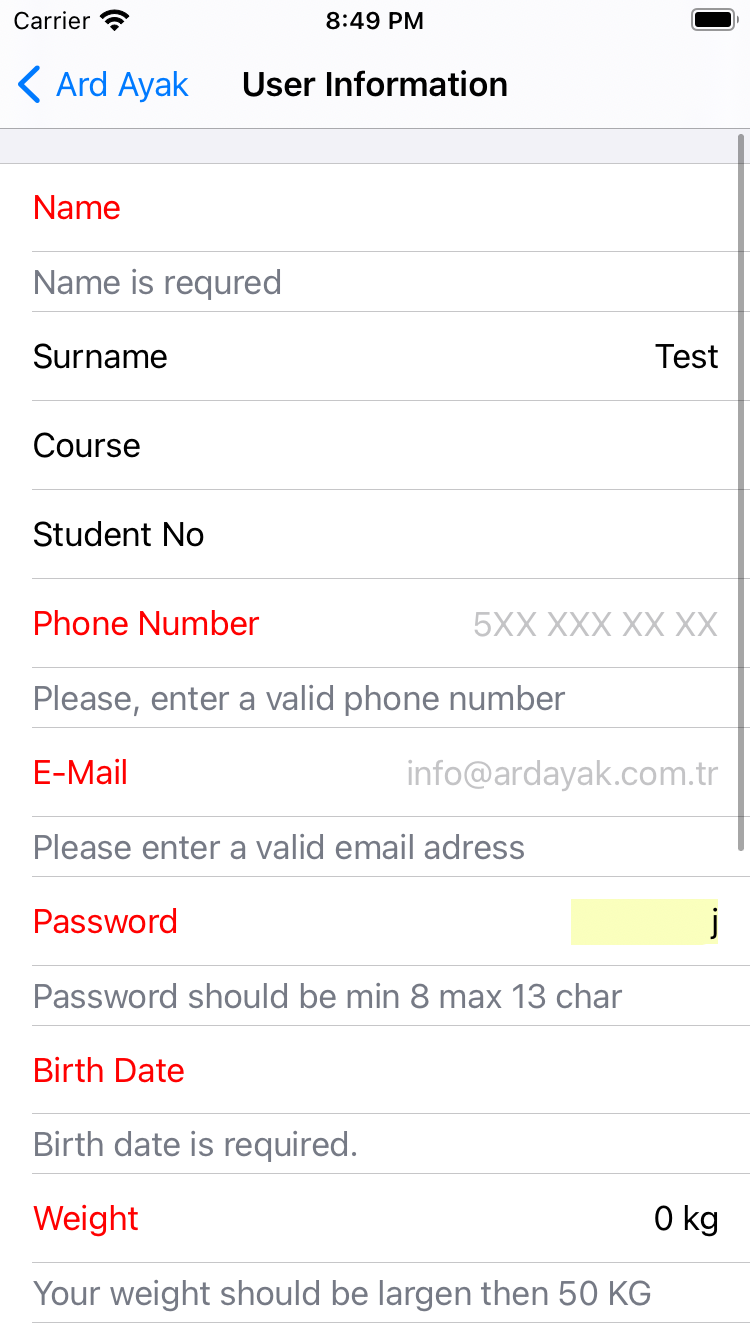
\includegraphics[width=.4\columnwidth]{KaanEksenMSc/figures/UserApplicationValidations.png}}
\caption{User application validations (iOS)}
\label{fig:UserApplicationValidations}
\end{figure}

Even though end-user documentation is created, client applications always consider user mistakes and misunderstandings. Therefore, input validation and feedback are implemented through the application. These validations include input type, max-min character, logical validations, and many more, shown in Figure \ref{fig:UserApplicationValidations}, to improve users' experience. In addition, user tutorials are also added to guide the user, which is shown in Figure \ref{fig:UserApplicationOnboarding}.

The image collection is a fundamentally similar process for both clients. This process includes taking a photo or taking it from the gallery. After that, since image sizes are different in different hardware, applications resize the image and transfer it in base64 format. Furthermore, file compression is used to reduce the traffic when transmitting the images from client to server. Deflate, a lossless compression format, is selected for compassion since it is a widely used open-source compression algorithm available in major operating systems. In addition, there is a file format validation on clients for gallery-selected images. 

\begin{figure}[htbp]
\centering
\fbox{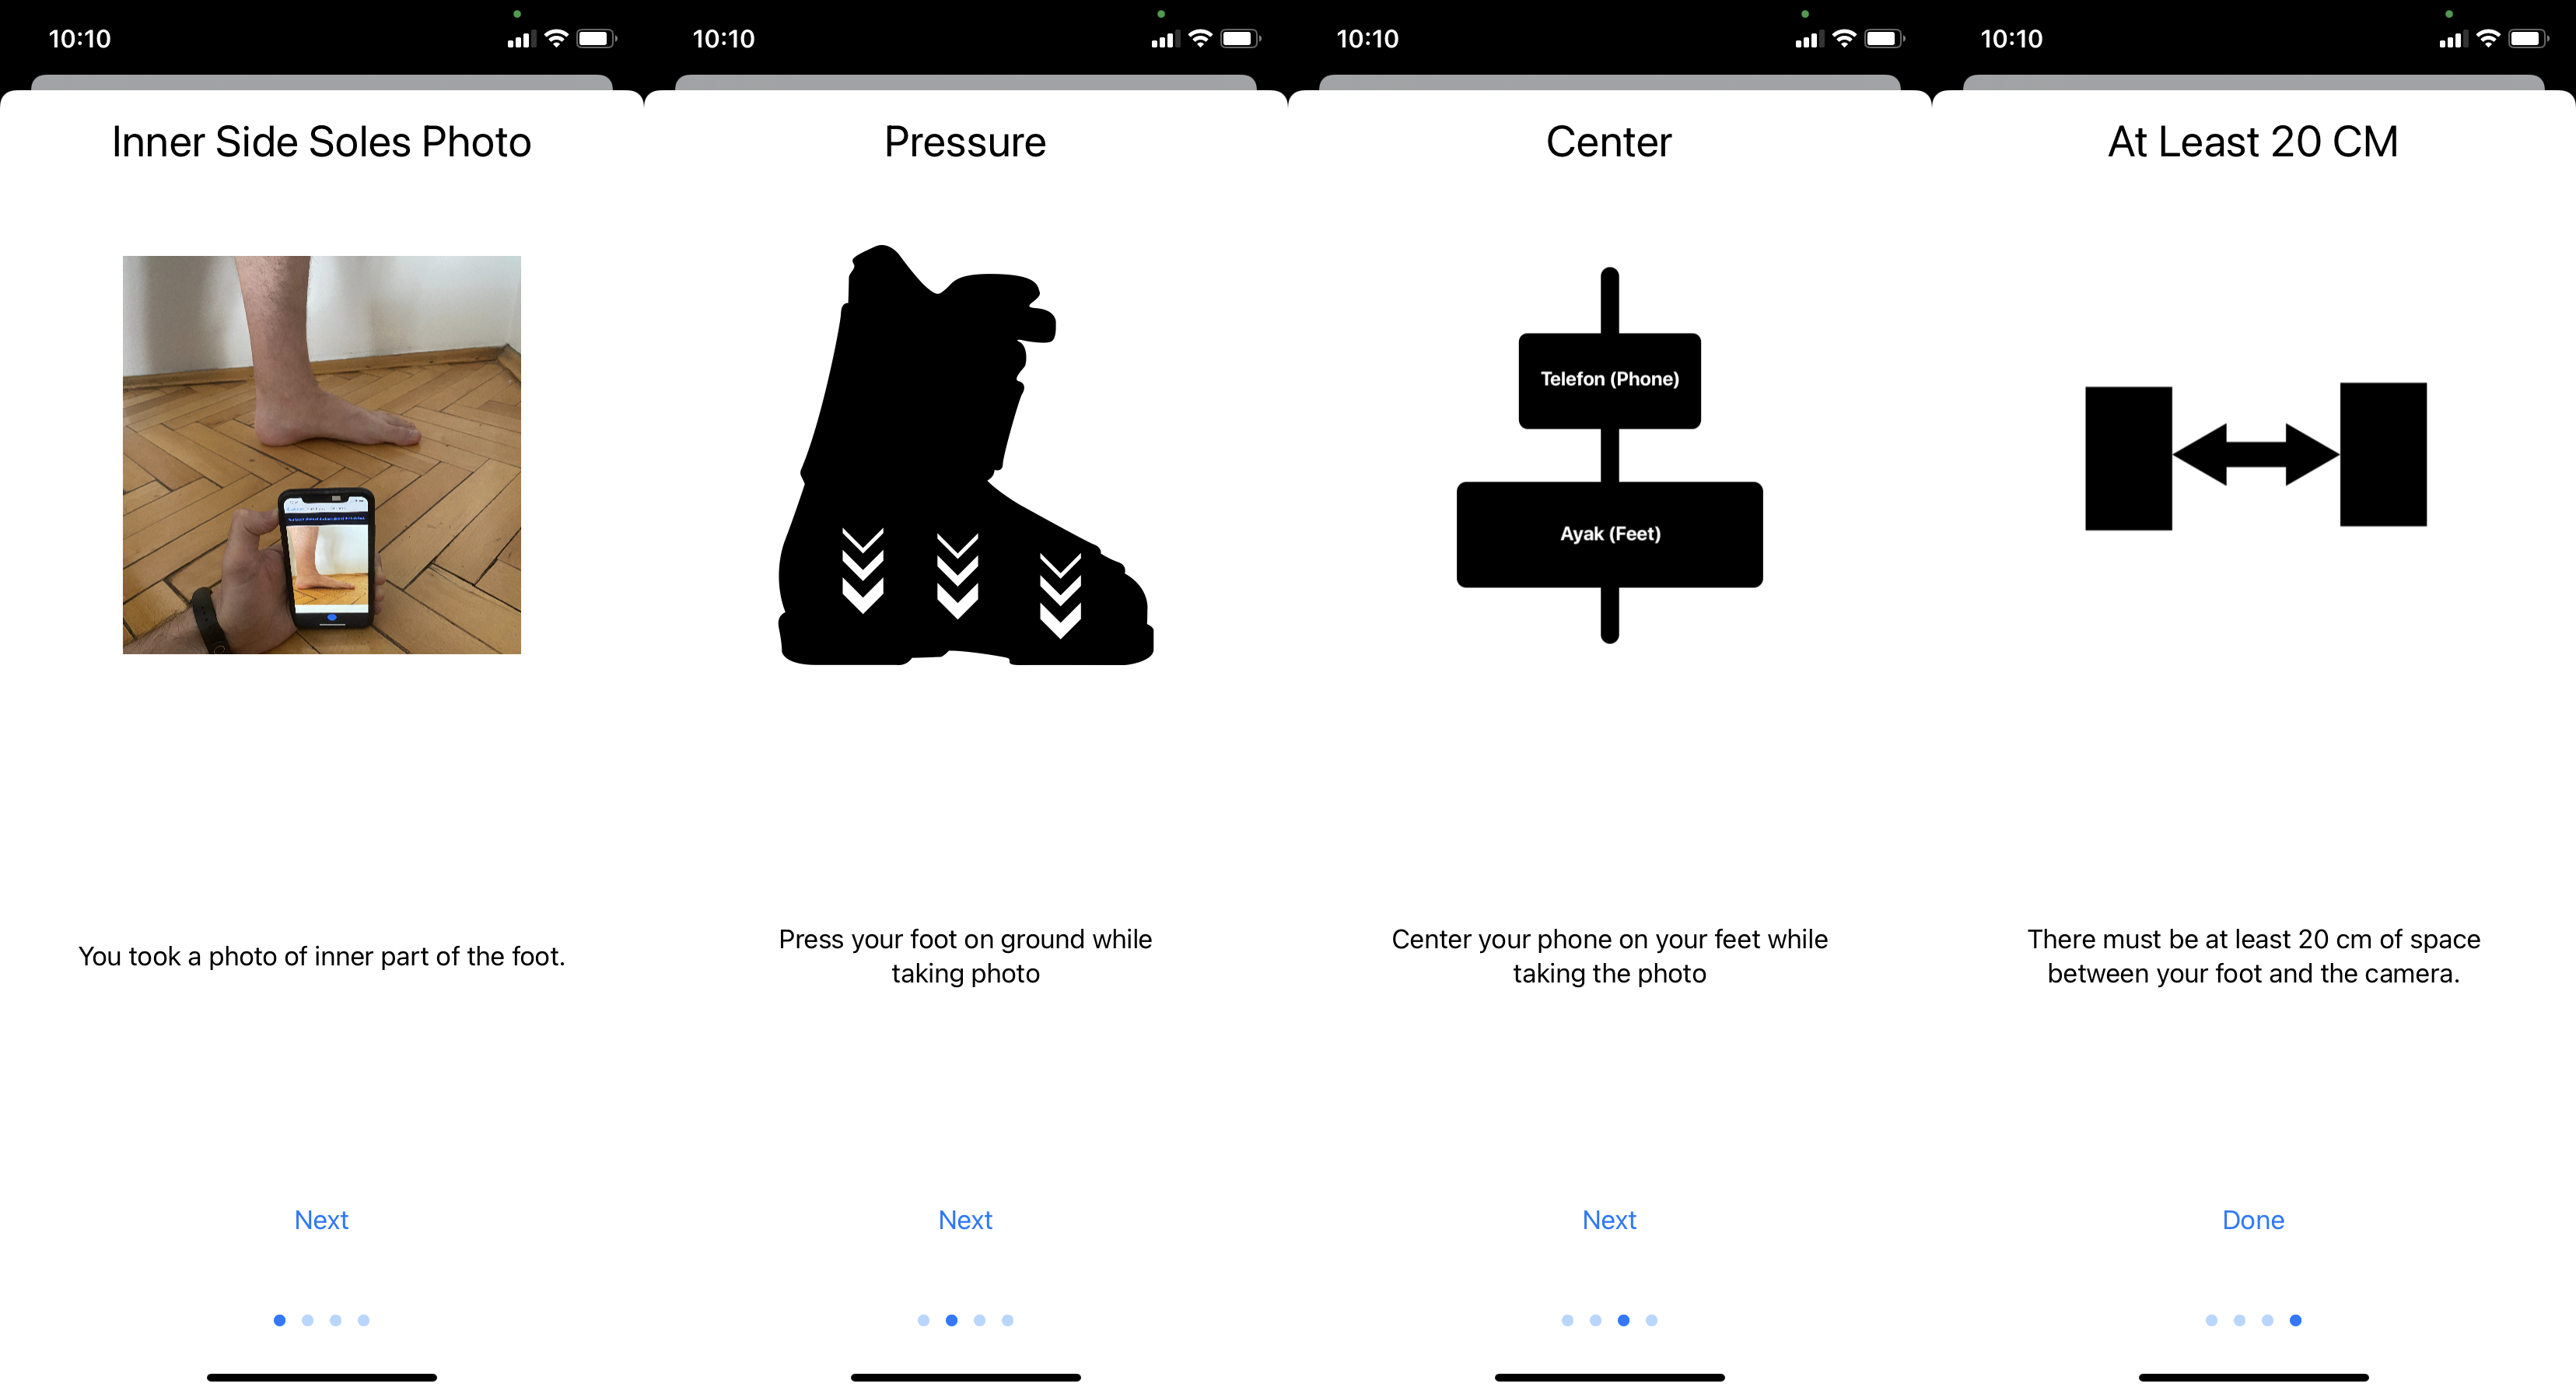
\includegraphics[width=.9\columnwidth]{KaanEksenMSc/figures/UserApplicationOnboarding.png}}
\caption{User application onboarding (iOS)}
\label{fig:UserApplicationOnboarding}
\end{figure}

The shooting angle and feet pressuring the ground during the photos shooting are essential for pes planus and pes cavus detection. Therefore onboarding is displayed (see Figure \ref{fig:UserApplicationOnboarding}) before each shooting. This onboarding shows a preview of how shooting should be and the state of the foot. As a result, this will reduce human-related errors furthermore. 

\begin{figure}[htbp]
\centering
\fbox{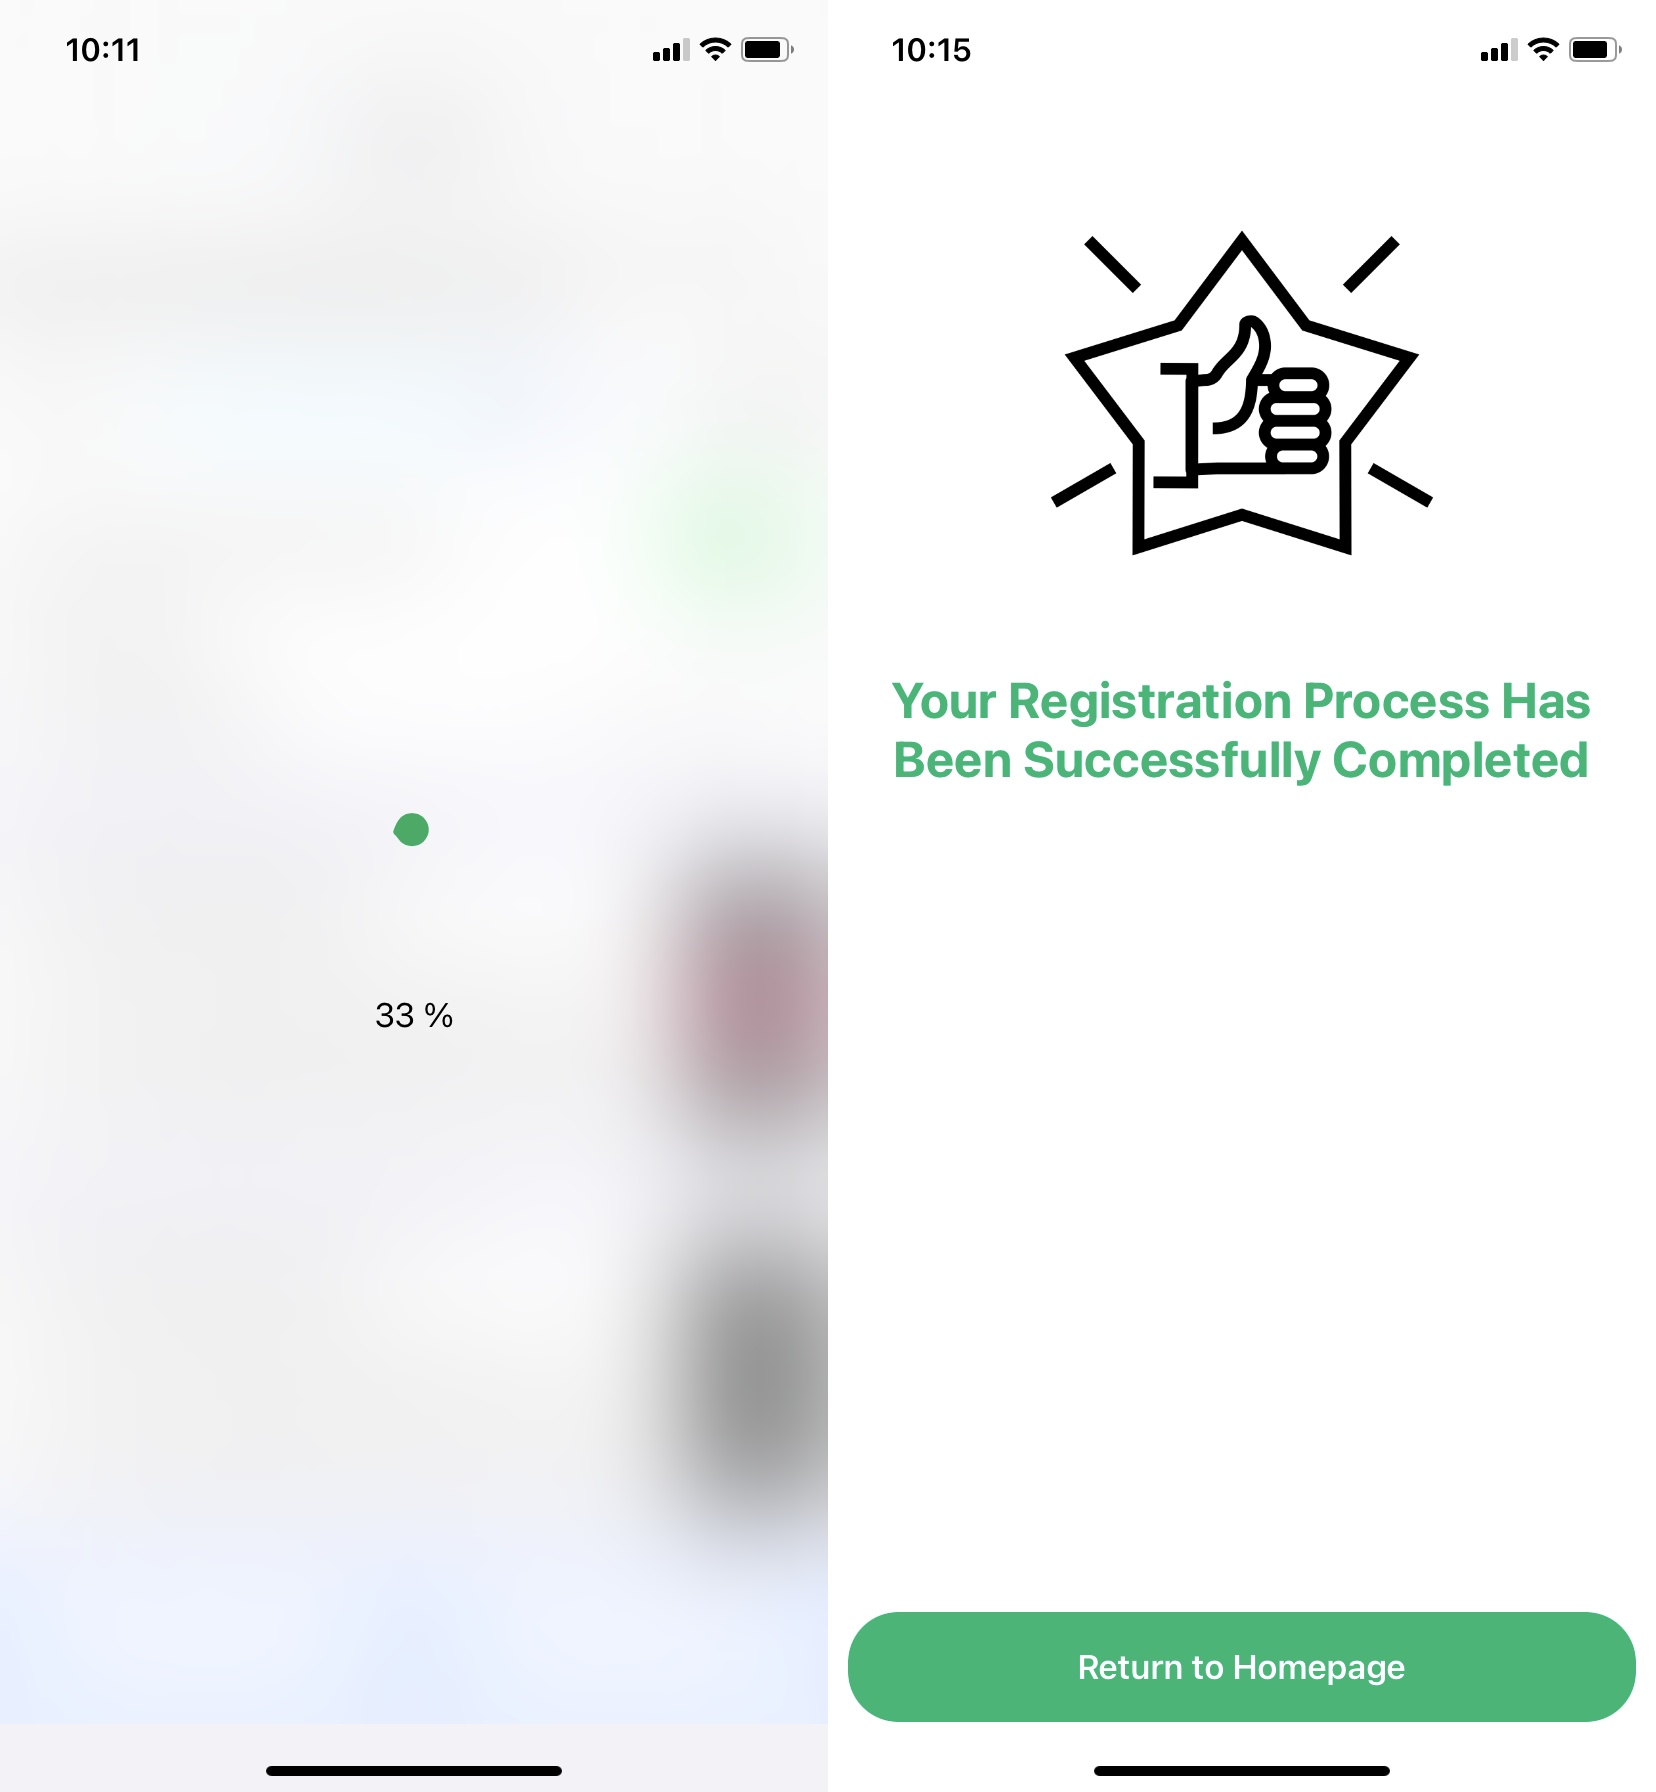
\includegraphics[width=.6\columnwidth]{figures/UserApplicationFeedback.png}}
\caption{User application feedback (iOS)}
\label{fig:UserApplicationFeedback}
\end{figure}

Feedbacks are one of the most critical aspects of the user experience. Therefore, multiple feedback mechanisms are developed in client applications to reduce communication errors. For example, since image uploading relatively takes more time than the other operations in the application, a progress bar with percentages is developed (see Figure \ref{fig:UserApplicationFeedback}). In addition, success screens are developed to indicate to users that the process is completed (see Figure \ref{fig:UserApplicationFeedback}).

The most important difference between iOS and Android processors is that some mobile phone models provide information other than raw image data during photo capture. For example, some of the Apple hardware contains LIDAR sensors. Therefore, the iOS client uses this hardware advantage and sends extra information to the service, which is the depth data. This depth information could be used to increase the accuracy of pre-diagnosis. In addition, depth data is converted to Point Cloud Data format before being transferred to the server for future updates for other systems.

Lastly, localization is one of the features of the client applications. Applications support multiple languages to increase usability in multiple regions in the world. In addition, supporting other languages would be straightforward as adding a new file to the application language file base. Furthermore, the client applications use operating system APIs to open the application in users' preferred language.

\subsection{Specialist Interface} \label{sec:SpecialistInterface}

The specialist interface is a web application whose primary purpose is to enable healthcare professionals to view patient data and diagnosis the patient based on the provided data. In the background, this process also improves the system by providing data to improve pre-diagnosis, which will be detailly discussed in the batch process. 

\begin{figure}[htbp]
\centering
\fbox{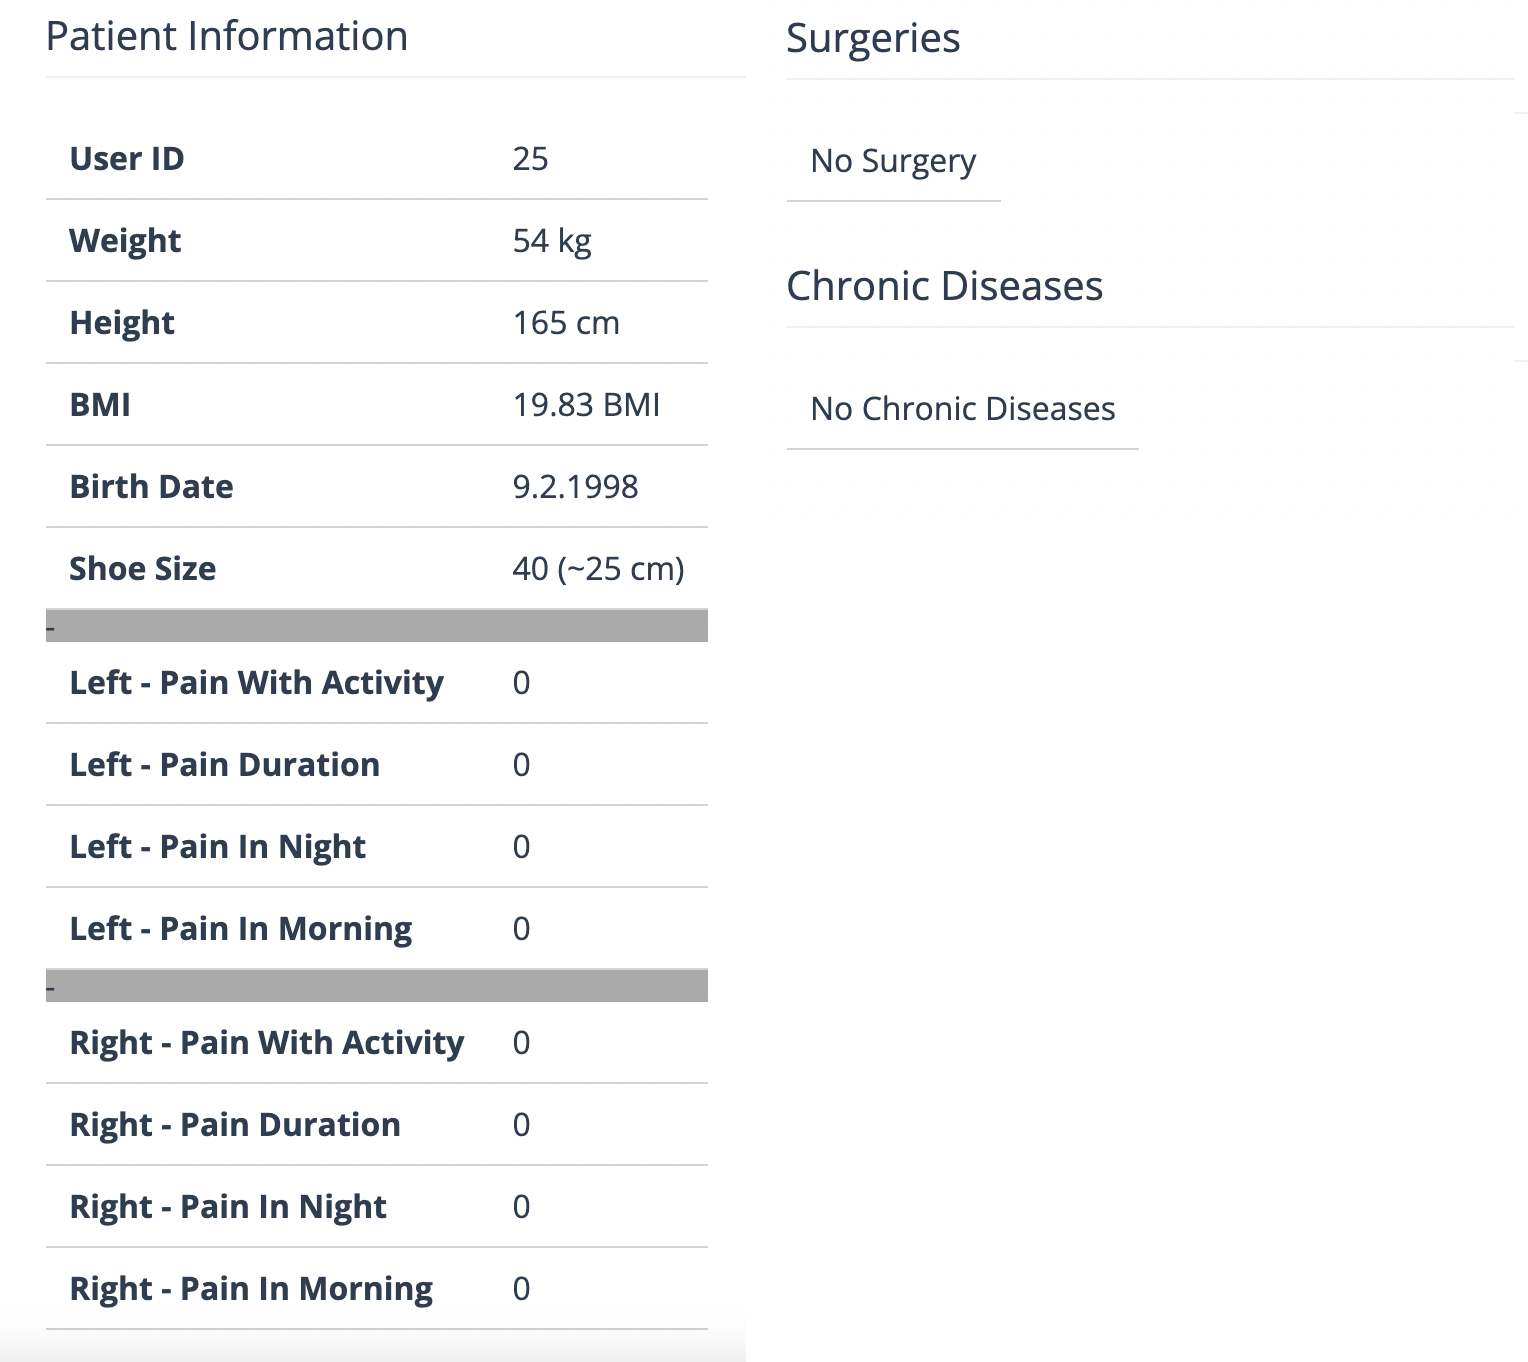
\includegraphics[width=.8\columnwidth]{figures/WebApplicationPatientInfo.png}}
\caption{Web application patient information}
\label{fig:WebApplicationPatientInfo}
\end{figure}

The specialist interface is designed to work in two cycles. In the first cycle, the system provides essential patient information such as age, foot size, surgeries, and chronic disease, shown in Figure \ref{fig:WebApplicationPatientInfo}. After validating initial information, healthcare professionals can set key decision-making points in images provided by patients, which will be used to calculate novel-approved foot indexes. 

\begin{figure}[htbp]
\centering
\fbox{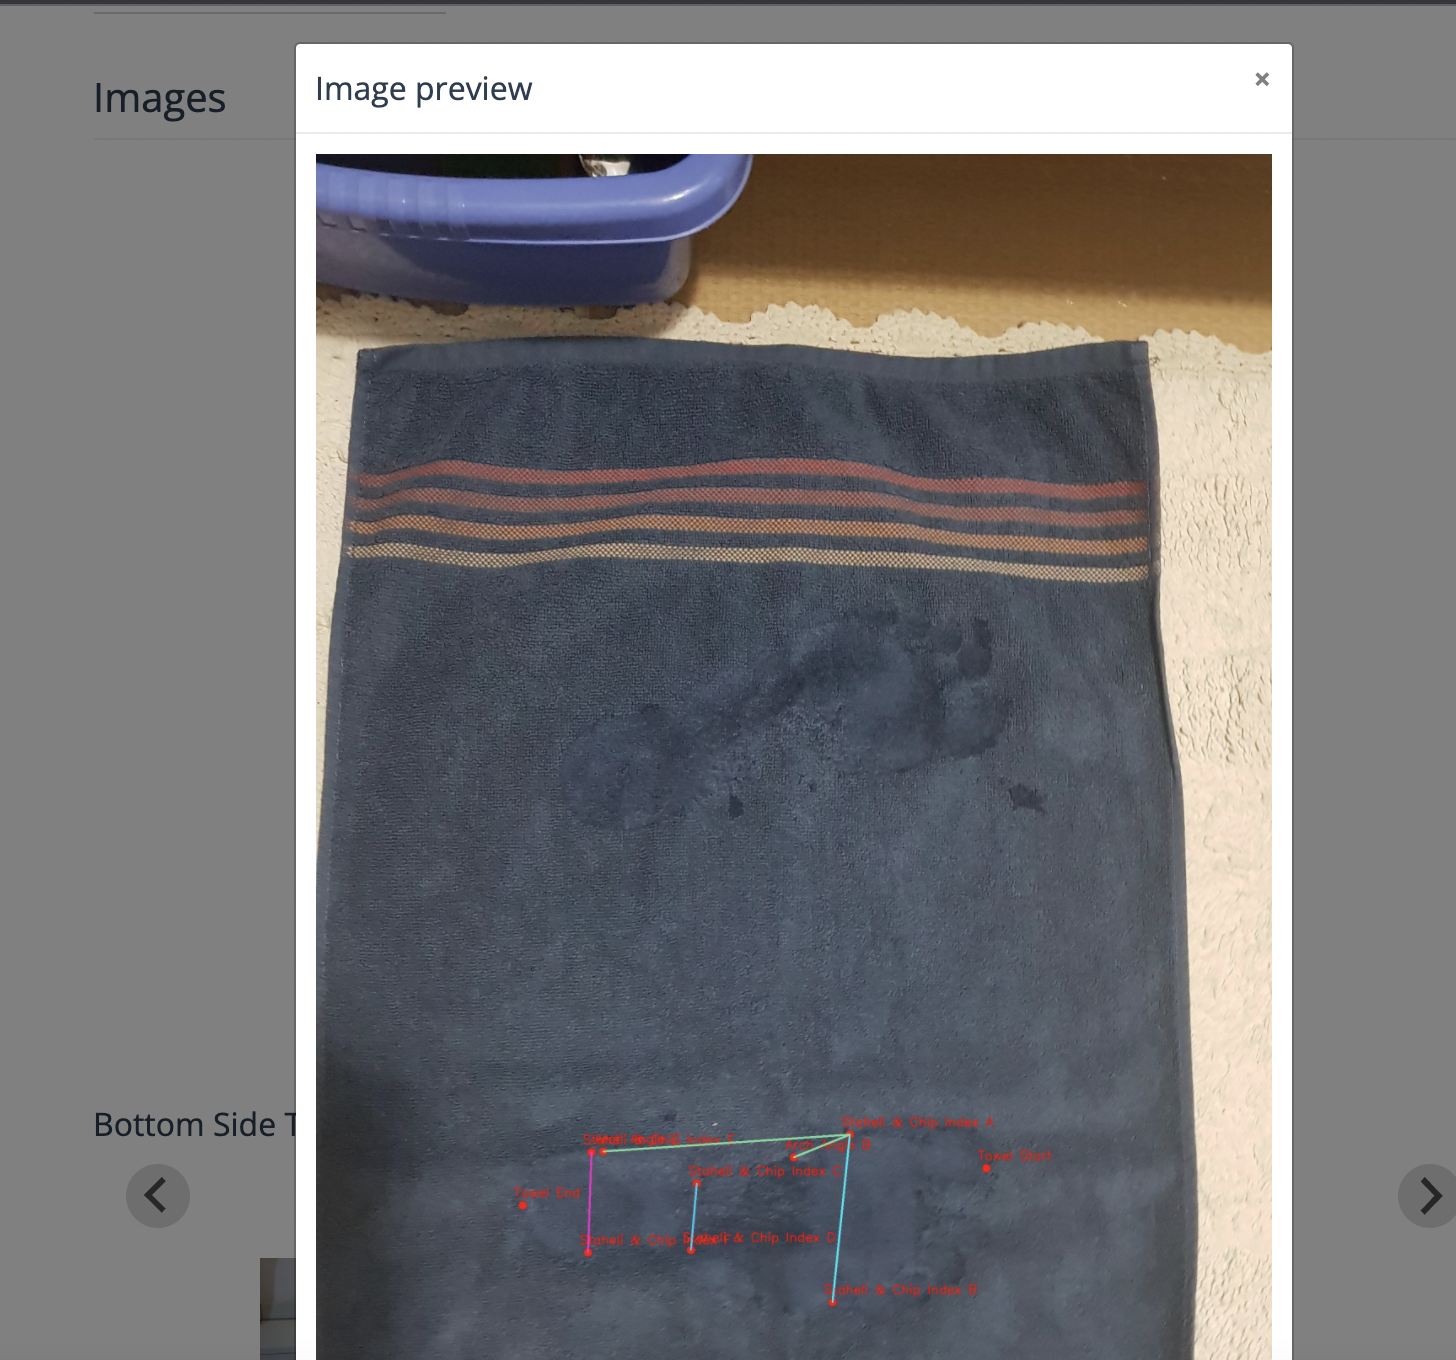
\includegraphics[width=.8\columnwidth]{KaanEksenMSc/figures/WebApplicationFootPoints.png}}
\caption{Web application critical foot points on image}
\label{fig:WebApplicationFootPoints}
\end{figure}

\begin{figure}[htbp]
\centering
\fbox{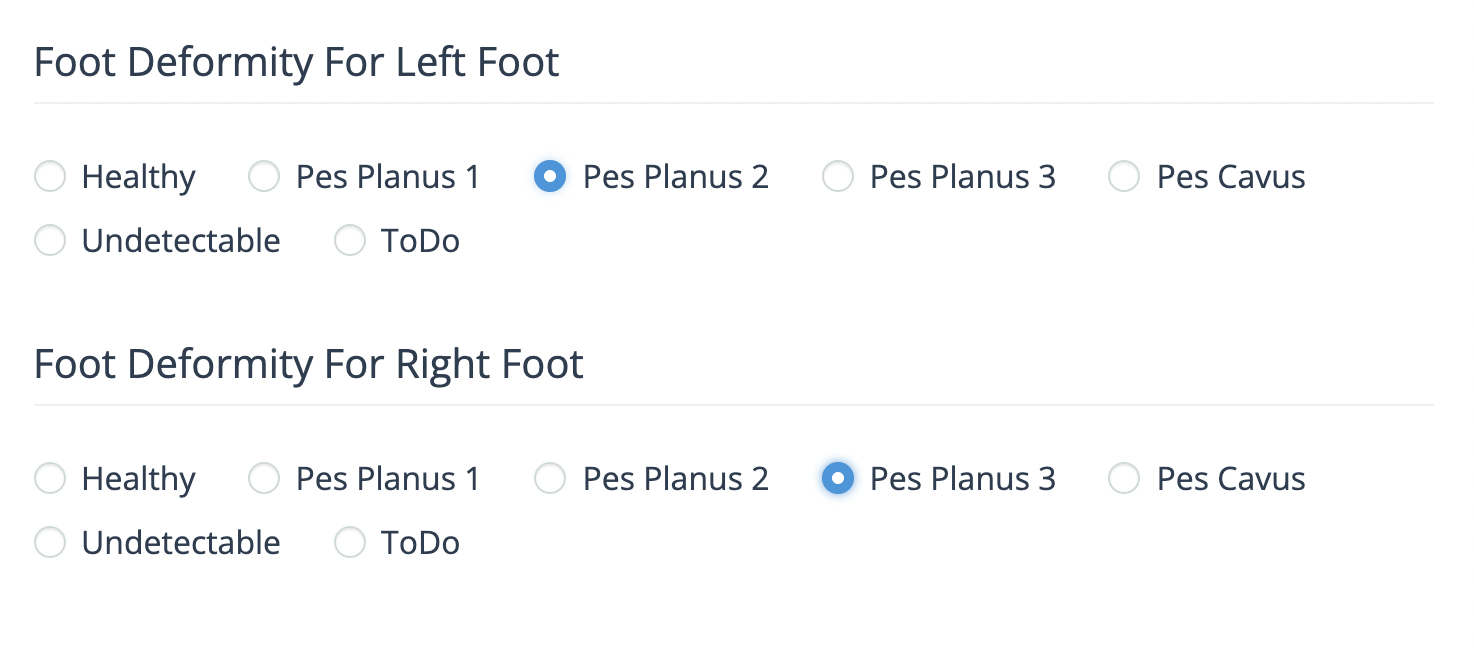
\includegraphics[width=.9\columnwidth]{KaanEksenMSc/figures/WebApplicationSetFootDeformity.png}}
\caption{Web application foot deformity options}
\label{fig:WebApplicationSetFootDeformity}
\end{figure}

The second cycle provides calculated results so that healthcare officials can make the final diagnosis of the patient's condition. Therefore, applications provide an overview of the patient information and display decision-making points in images to ensure they are correct (see Figure \ref{fig:WebApplicationFootPoints}). Healthcare officials can redo the point set or diagnose the patient (see Figure \ref{fig:WebApplicationSetFootDeformity}). In addition, in case of unusable images, there is an option that asks the user to re-upload foot pictures.

\begin{figure}[htbp]
\centering
\fbox{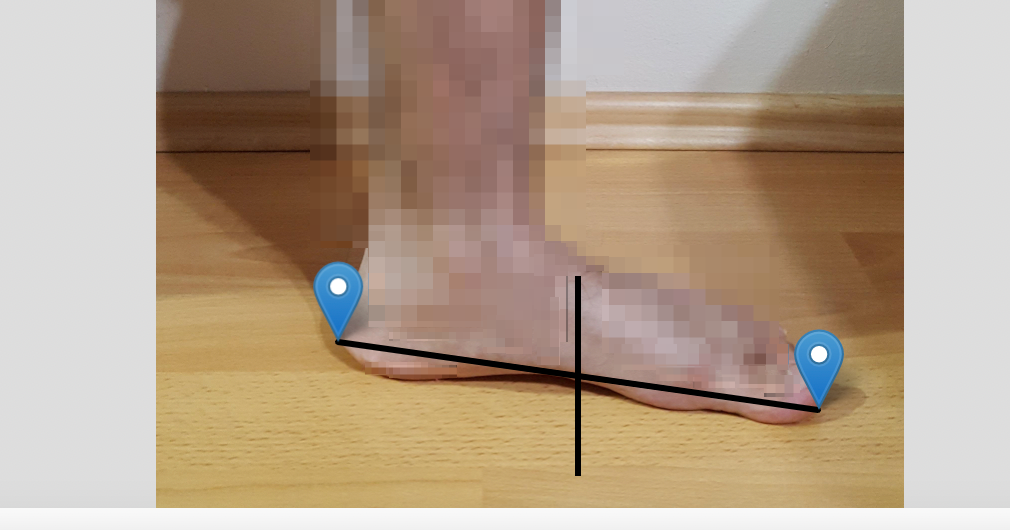
\includegraphics[width=.6\columnwidth]{KaanEksenMSc/figures/WebApplicationCriticalPointAssistance.png}}
\caption{Web application critical point assistance}
\label{fig:WebApplicationCriticalPointAssistance}
\end{figure}

The web application contains validations to ensure current diagnosis. Thus, the system ensures that all the critical points are set in the initial cycle. The second cycle provides that human-related errors are eliminated, such as wrongly placed points. 

\begin{figure}[htbp]
\centering
\fbox{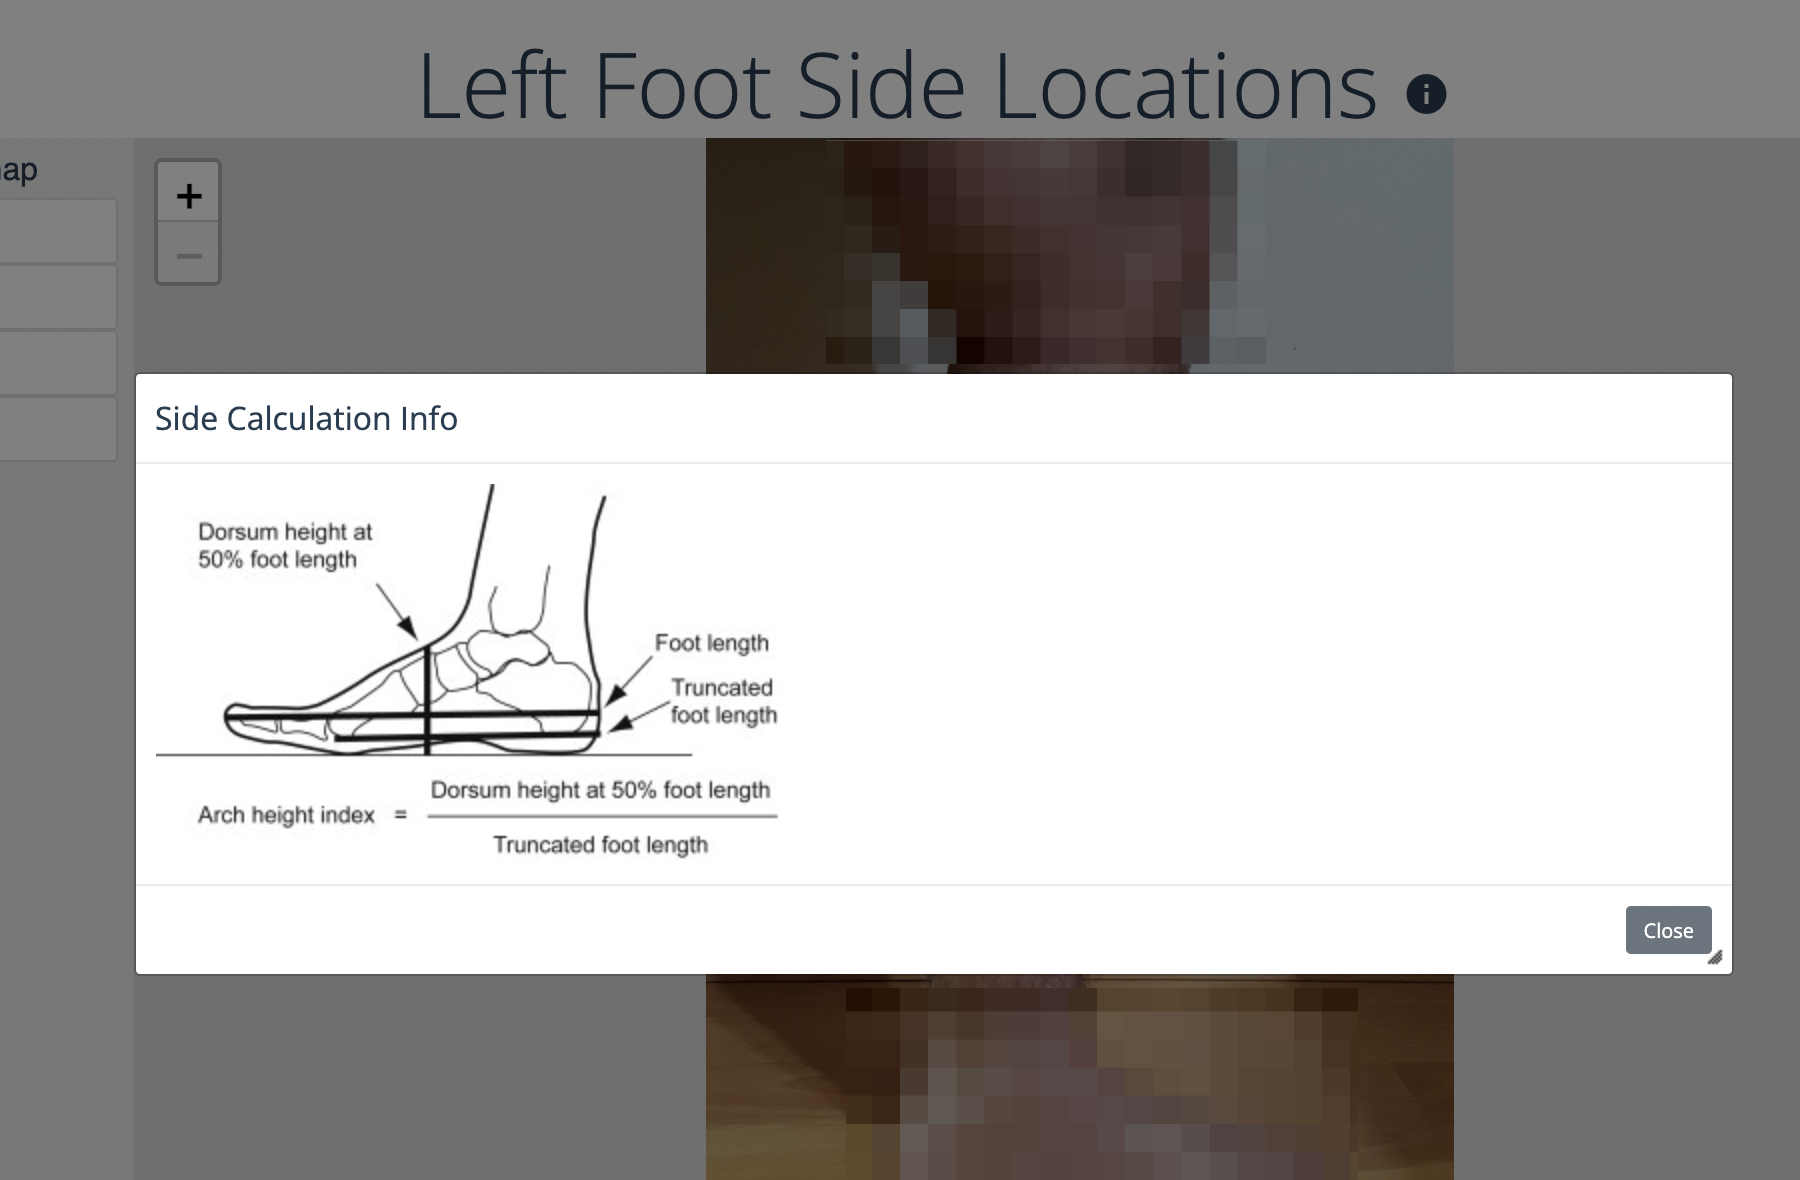
\includegraphics[width=.6\columnwidth]{KaanEksenMSc/figures/WebApplicationInformationBoxes.png}}
\caption{Web application information boxes}
\label{fig:WebApplicationInformationBoxes}
\end{figure}

In addition, The web application also provides helper functionalities to healthcare workers such as critical point assistance and information boxes. For example, the arch height index requires finding the center of the points therefore the critical point assistance displays (see Figure \ref{fig:WebApplicationCriticalPointAssistance}) the center of the points provided by the health professionals. Another example is that information boxes provide simple reminders about indexes (see Figure \ref{fig:WebApplicationInformationBoxes}).

\subsection{Services And Batch Process} \label{sec:StudyIServicesAndBatchProcess}
The application consists of two services: web and client application service. This structure provides scalability and security. Therefore, one service deals with end-user interactions and data transmission. At the same time, web service provides healthcare professionals and batch processes. With this separation, each service is placed in different layers. Therefore, this makes it possible that only client application services have internet access, increasing the web application security by limiting internet access. In addition, this will provide more hardware-intensive operations (image processing, deep learning) to other physical servers. 

Client application services adopt the microservice architecture for scalability and respond quickly to requirements. Furthermore, to prevent unauthorized access JWT (RFC 7519) is used. Lastly, all communications have been done by HTTP protocol with an SSL (RFC 6101). 

The batch process is the system's core, where the pre-diagnosis is done. The pre-diagnosis computation has three main steps: finding the region of interest, image pre-processing, and detection. Afterward, results are shared with the appropriate application and recorded in the database. In the following paragraphs, each step is detailly explained.

The initial step requires finding the foot in the image, also called the region of interest (ROI). Since all the data is collected unsupervised, the foot can be anywhere in the image. Therefore, roughly locating the foot for detail processing is essential. Deep learning algorithms are excellent in object recognition, but they require a vast amount of data to achieve this type of accuracy, so using deep learning algorithms for pre-diagnosis is close to impossible with the current dataset. As a result, the study uses pre-trained deep learning human detection algorithms to get a rough location of the foot.

\begin{figure}[htbp]
\centering
\fbox{\includegraphics[width=.7\columnwidth]{KaanEksenMSc/figures/DeepLearningTest.jpeg}}
\caption{Deep learning test - DeepLab, FCN, YOLO, Skin, MIDAS (left to right)}
\label{fig:DeepLearningTest}
\end{figure}

The foot detection rate of the algorithms might not be as accredited as the announced results because most public datasets contain an entire human body other than a barefoot. Therefore, multiple deep learning networks such as YOLO, MIDAS, FCN Resnet 101, DeepLabV3 have been tested in small datasets for best results (see Figure \ref{fig:DeepLearningTest}).

\begin{figure}[htbp]
\centering
\fbox{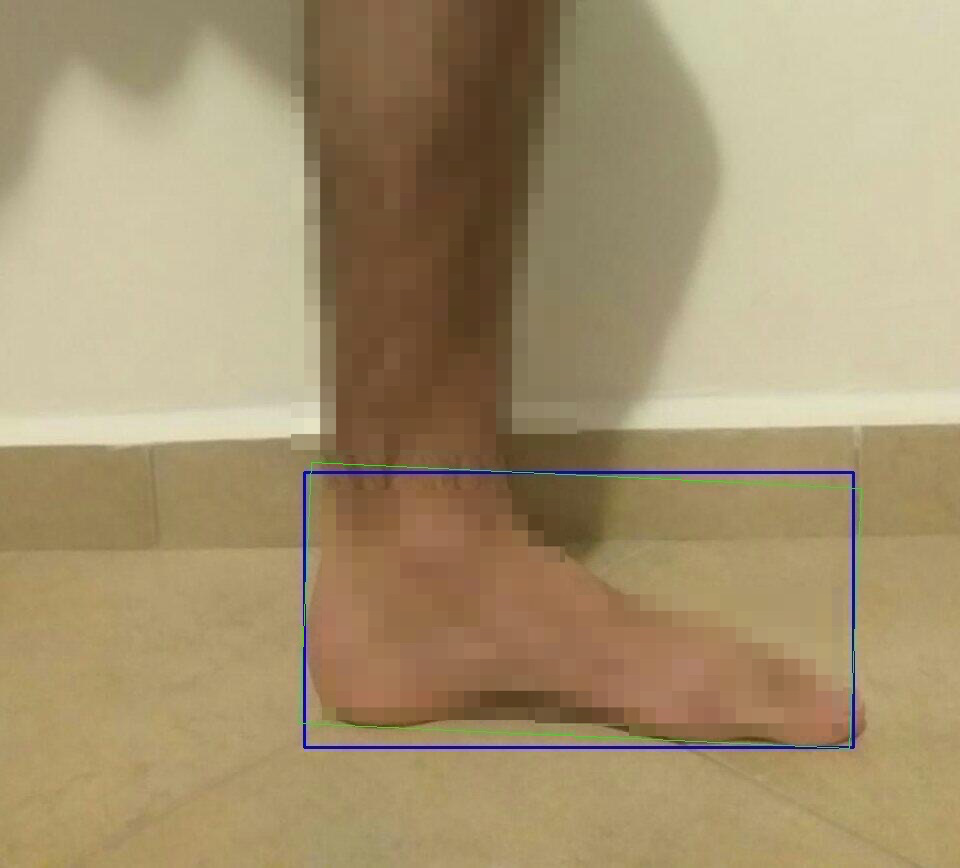
\includegraphics[width=.6\columnwidth]{KaanEksenMSc/figures/BatchProcessMinimumBoundingBox.png}}
\caption{Batch process minimum bounding box (green line)}
\label{fig:BatchProcessMinimumBoundingBox}
\end{figure}

In addition, skin detection algorithms are also tested. Initially, the YCbCr color space-based skin detection algorithm was applied, but detection results have been unsuccessful in some lighting conditions. Therefore, the zero-sum game-based skin detection algorithm proposed by Dahmani et al. \cite{dahmani2020zero} is also tested (see Figure \ref{fig:DeepLearningTest}). Overall, the best performance has been achieved by DeepLabV3.

The second step deals with image preparation. After potential barefoot is detected, a minimum area rectangle is calculated because the foot's location and angle might not be as accurate as demonstrated in the usage document. Therefore, perspective transformation is applied with the minimum area rectangle, eliminating potential angle problems (see Figure \ref{fig:BatchProcessMinimumBoundingBox}). In addition, this will move any foot on the image to the left corner of the image, which will ease the calculations.

\begin{figure}[htbp]
\centering
\fbox{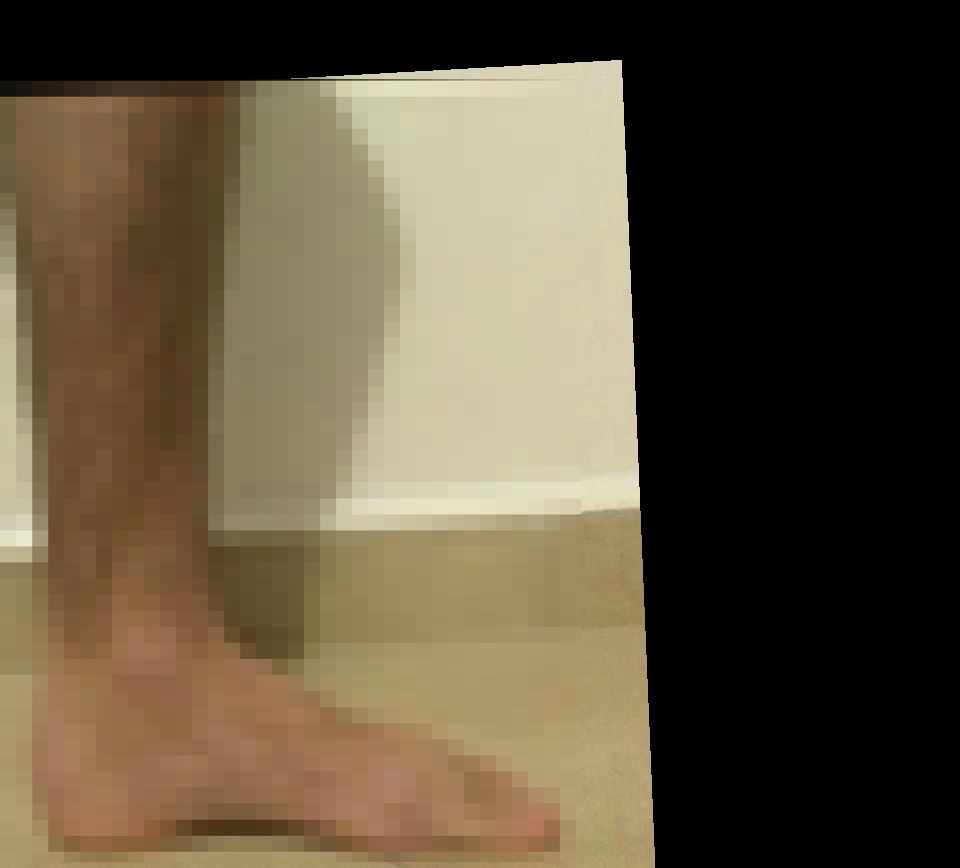
\includegraphics[width=.6\columnwidth]{KaanEksenMSc/figures/BatchProcessPerspectiveTransformation.png}}
\caption{Batch process perspective transformation}
\label{fig:BatchProcessPerspectiveTransformation}
\end{figure}

After the perspective transformation (see Figure \ref{fig:BatchProcessPerspectiveTransformation}), grayscale is required for edge detection algorithms. Therefore, RGB color space is converted to HSL because HSL has a separate lightness channel that can be eliminated. After all, lightness is unrelated to foot detection. The S channel was selected for the grayscale conversation since S performed better than H in the small dataset.

\begin{figure}[htbp]
\centering
\fbox{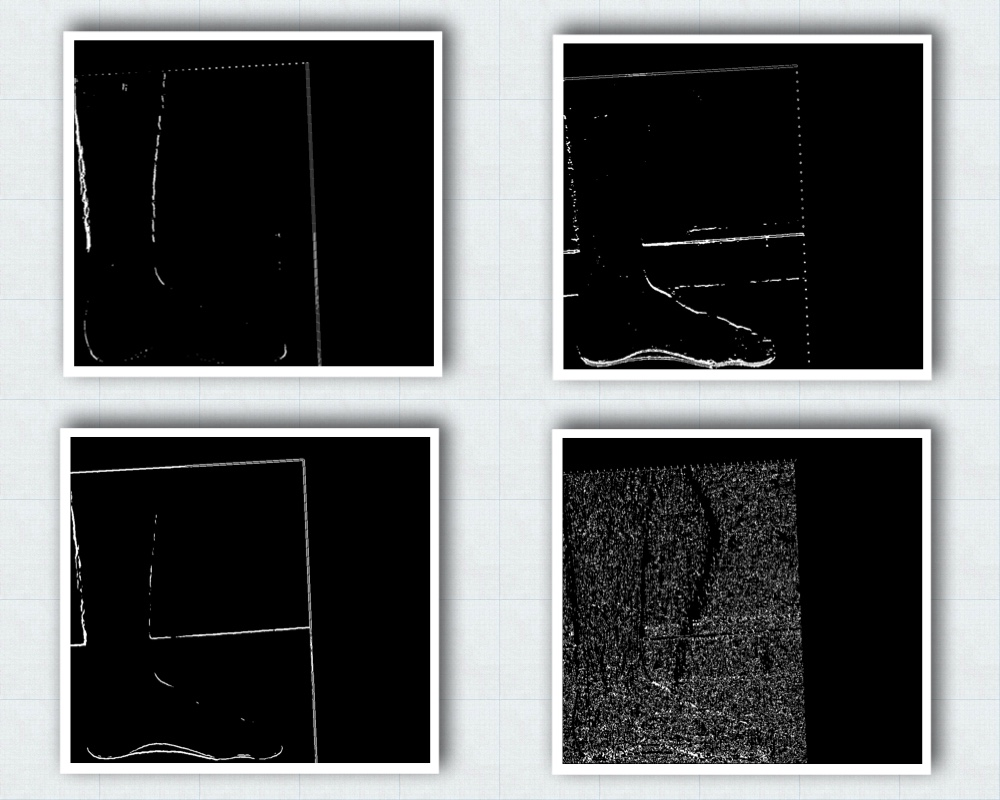
\includegraphics[width=.6\columnwidth]{KaanEksenMSc/figures/BatchProcessSobelOutput.jpg}}
\caption{Batch Process - Sobel - Absolute Gradient X, Absolute Gradient Y, Magnitude Gradient, Directional Gradient - Left To Right}
\label{fig:BatchProcessSobelOutput}
\end{figure}

The final stage includes edge detection and functionalization of the sole. The sobel algorithm is selected for edge detection with four different approaches with threshold values (see Figure \ref{fig:BatchProcessSobelOutput});

\begin{itemize}
  \item Applying an absolute gradient with the X direction
  \item Applying an absolute gradient with the Y direction
  \item Applying a magnitude gradient
  \item Applying a directional gradient with an angle threshold 
\end{itemize}

\begin{figure}[htbp]
\centering
\fbox{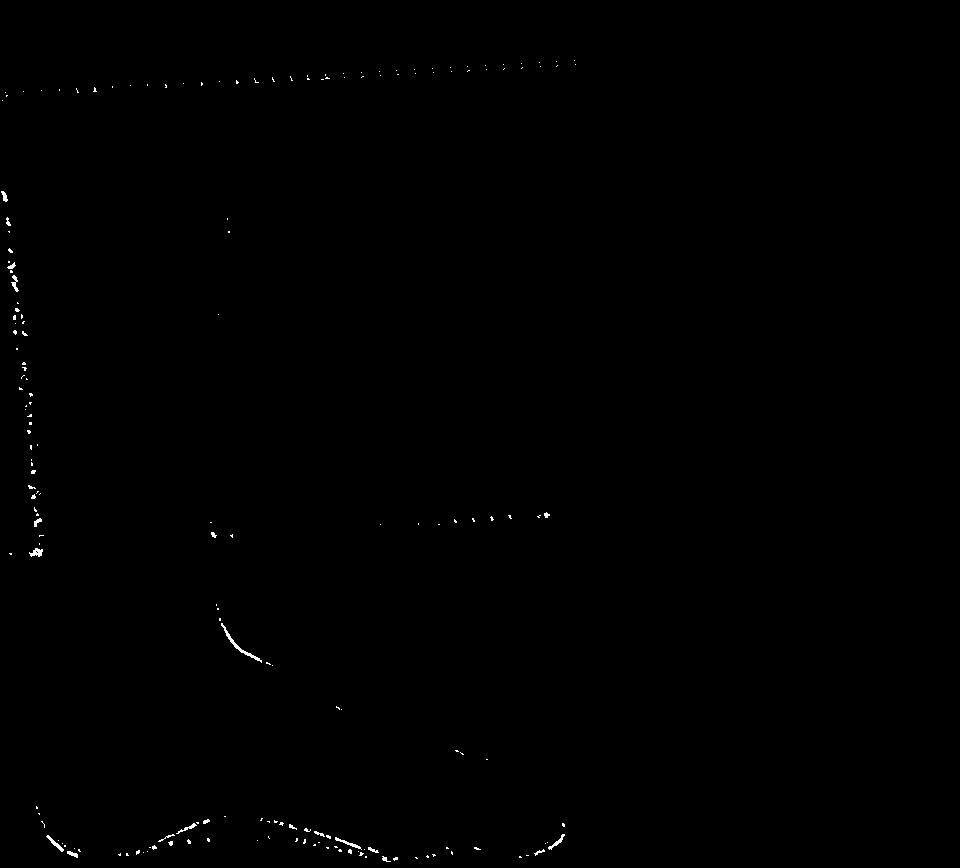
\includegraphics[width=.6\columnwidth]{KaanEksenMSc/figures/BatchProcessEdge.jpeg}}
\caption{Batch process Sobel combined}
\label{fig:BatchProcessEdge}
\end{figure}

After applying each configuration to the transformed image, results are merged into one with the algorithm \ref{alg:CombinedSobelResults}, which reduces unwanted pixels (see Figure \ref{fig:BatchProcessEdge}). 

\begin{figure}[htbp]
\centering
\fbox{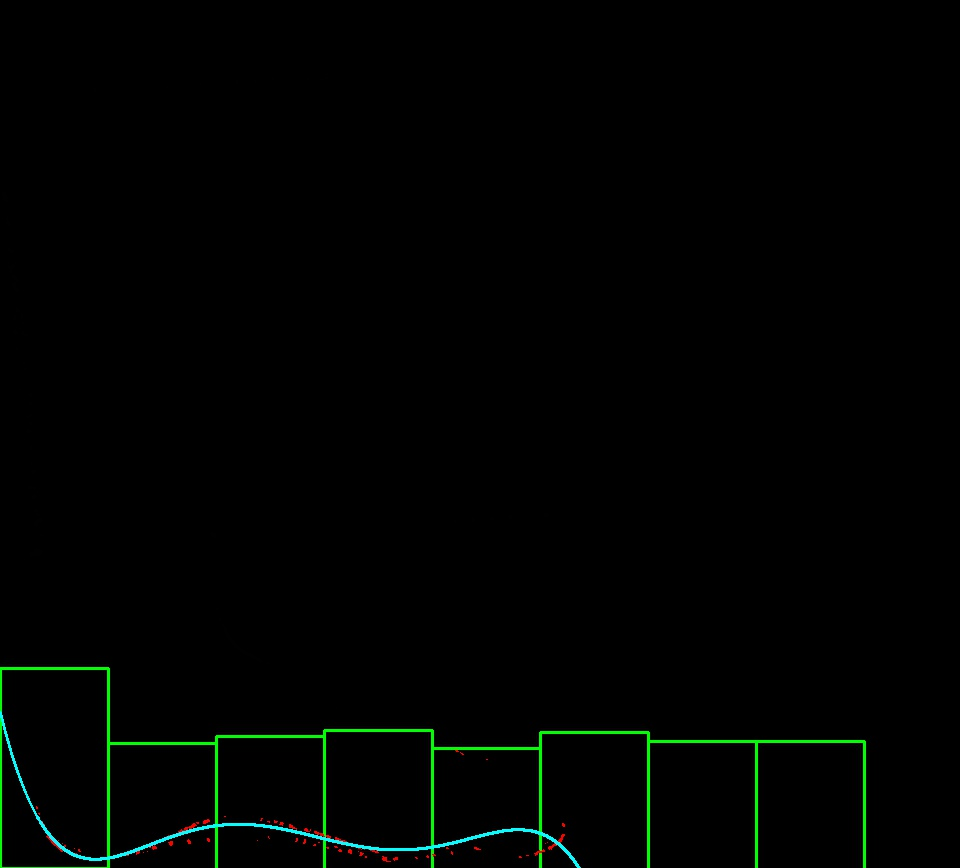
\includegraphics[width=.6\columnwidth]{KaanEksenMSc/figures/BatchProcessLine.jpeg}}
\caption{Batch process polynomial function}
\label{fig:BatchProcessLine}
\end{figure}

After the edges are extracted, polynomial regression is applied to generate the polynomial function of the solo. In addition, the fifth-order (quintic) polynomial function is selected to get matching curves of the solo. Furthermore, polynomial regression is applied with predefined windows(see Figure \ref{fig:BatchProcessLine}) because curve transitions will become smoother.

\begin{algorithm}
\caption{Merging Sobel results}\label{alg:CombinedSobelResults}
\begin{algorithmic}

\STATE $ABS_X \gets Absolute Gradient X$
\STATE $ABS_Y \gets Absolute Gradient Y$
\STATE $MAG \gets Magnitude Gradient$
\STATE $DIR \gets Directional Gradient$

\FORALL{$pixcel\in image$}
    \STATE $pixcel \gets (ABS_X \AND ABS_Y) \OR (MAG \AND DIR)$
\ENDFOR

\end{algorithmic}
\end{algorithm}

Critical locations on the foot will be located based on the solo function. For example, the metatarsal point is based on the solo function's second increase. In addition, The bottom-left and bottom-right positions of the foot will be located with the solo function and minimum bounding box.

\subsection{Database} \label{sec:StudyIDatabase}

MySQL was selected for the primary database because it provides a high degree of data integrity. In addition, the following reasons were also considered in selection: the data structure is not changing frequently, a relatively contains a small amount of data (a small percentage of users), and most importantly, data require a high degree of data integrity and security.

The database design (see Figure \ref{fig:DatabaseGeneralView}) was carried out within the drafts revealed due to the requirement analysis. In this process, tables were created based on the Normal forms, which were created to minimize errors and improve designs. Initially, three Normal forms were considered in the design: the first, second, and third normal forms. After that, fourth and fifth normal forms (Fifth Normal Form, 5NF) were also considered, based on the concepts of multivalued and join dependencies, respectively. Finally, all the de-normalization forms were taken into consideration during the database design.

The database was divided into eight major table groups based on usage and connections: ScanFileInfo, FootScan, File, Training, DiseaseHistory, User, Survey, and Diagnosis. Those groups help us understand the concept more clearly (see Figure \ref{fig:DatabaseGeneralView}). 

\begin{figure}[htbp]
\centering
\fbox{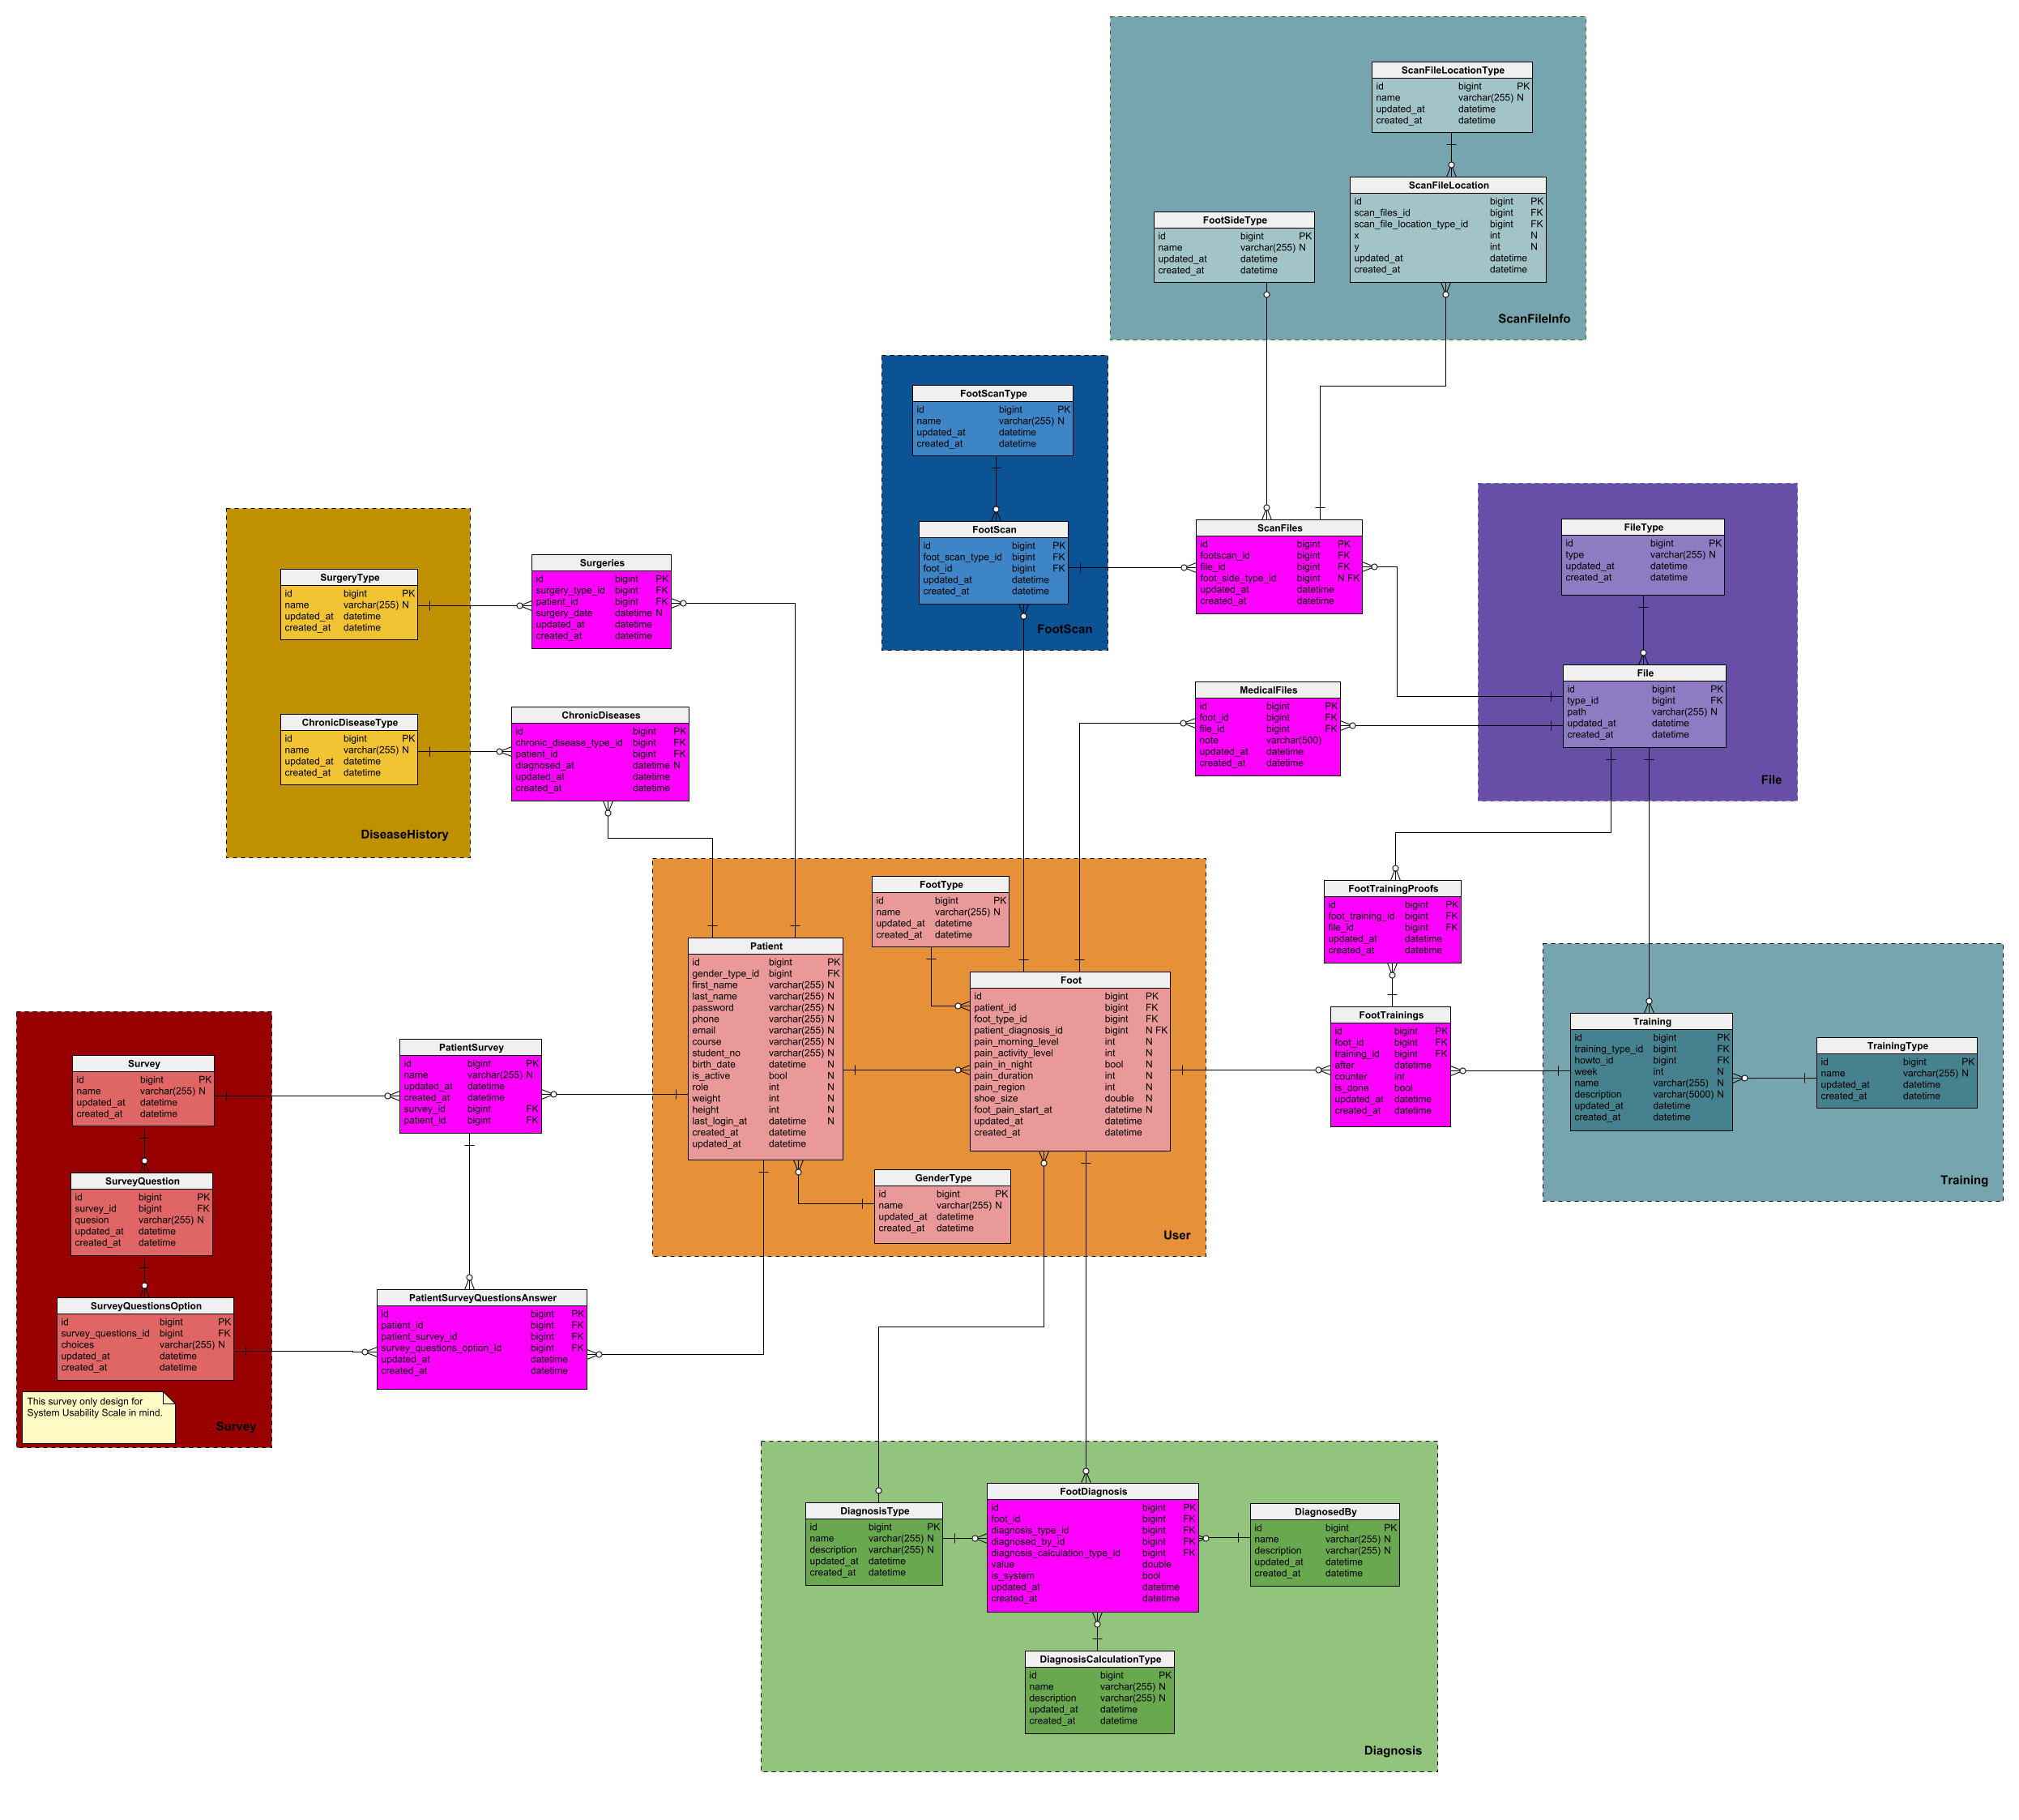
\includegraphics[width=1.0\columnwidth]{KaanEksenMSc/figures/DatabaseGeneralView.png}}
\caption{General view of database}
\label{fig:DatabaseGeneralView}
\end{figure}

User table group explicitly were designed for user and its components consist of patient, foot, foot type, and gender (see Figure \ref{fig:DatabaseUser}). In addition, users were had roles that help generalize the table, such as healthcare specialists or patients. Furthermore, foot type was added for patients with different conditions, such as a prosthetic foot.

\begin{figure}[htbp]
\centering
\fbox{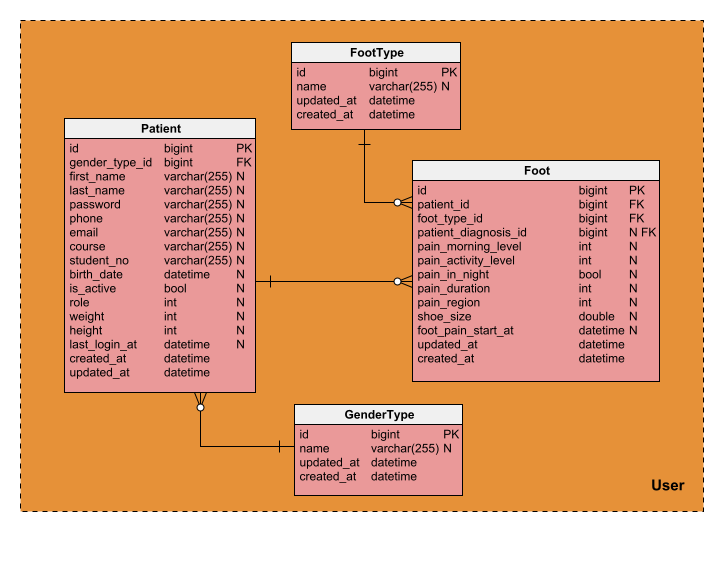
\includegraphics[width=.7\columnwidth]{KaanEksenMSc/figures/DatabaseUser.png}}
\caption{Database user group table}
\label{fig:DatabaseUser}
\end{figure}

The diagnosis table group focuses on foot diagnosis and detailed calculations methods (see Figure \ref{fig:DatabaseDiagnosis}). The foot may have multiple diagnoses from multiple healthcare specialists or the system. In addition, diagnoses calculation details can be recorded, such as the Staheli arch index.

\begin{figure}[htbp]
\centering
\fbox{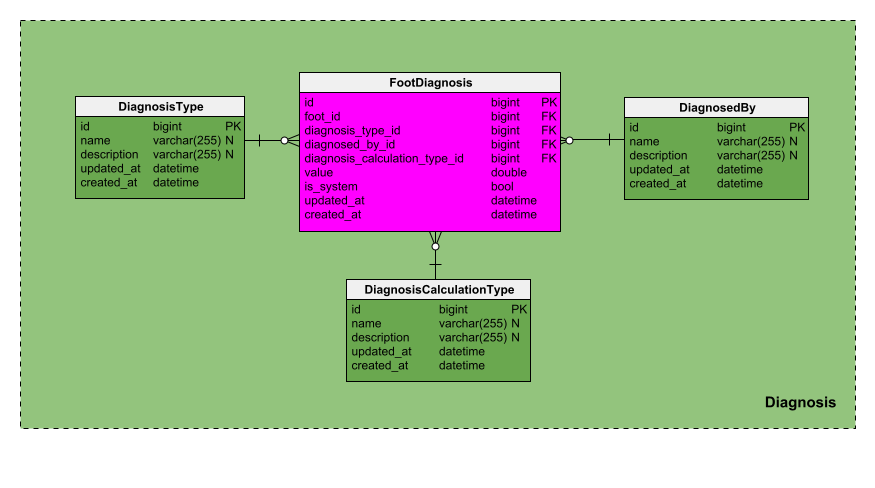
\includegraphics[width=.9\columnwidth]{KaanEksenMSc/figures/DatabaseDiagnosis.png}}
\caption{Database diagnosis group table}
\label{fig:DatabaseDiagnosis}
\end{figure}

The ScanFileInfo, FootScan, File table groups were designed to record patient assets according to the examination type (see Figure \ref{fig:DatabaseFiles}). FootScan records examination type such as Foot Deformity or Rom Measurement. Each examination can have unlimited images recorded in the ScanFiles table with a type such as Bottom, Back Side. Each image might have essential locations recorded in the ScanFileLocation table, such as the side thumb. In addition, file information such as file system locations is recorded in the File table, and each file contains a file type for processing.

\begin{figure}[htbp]
\centering
\fbox{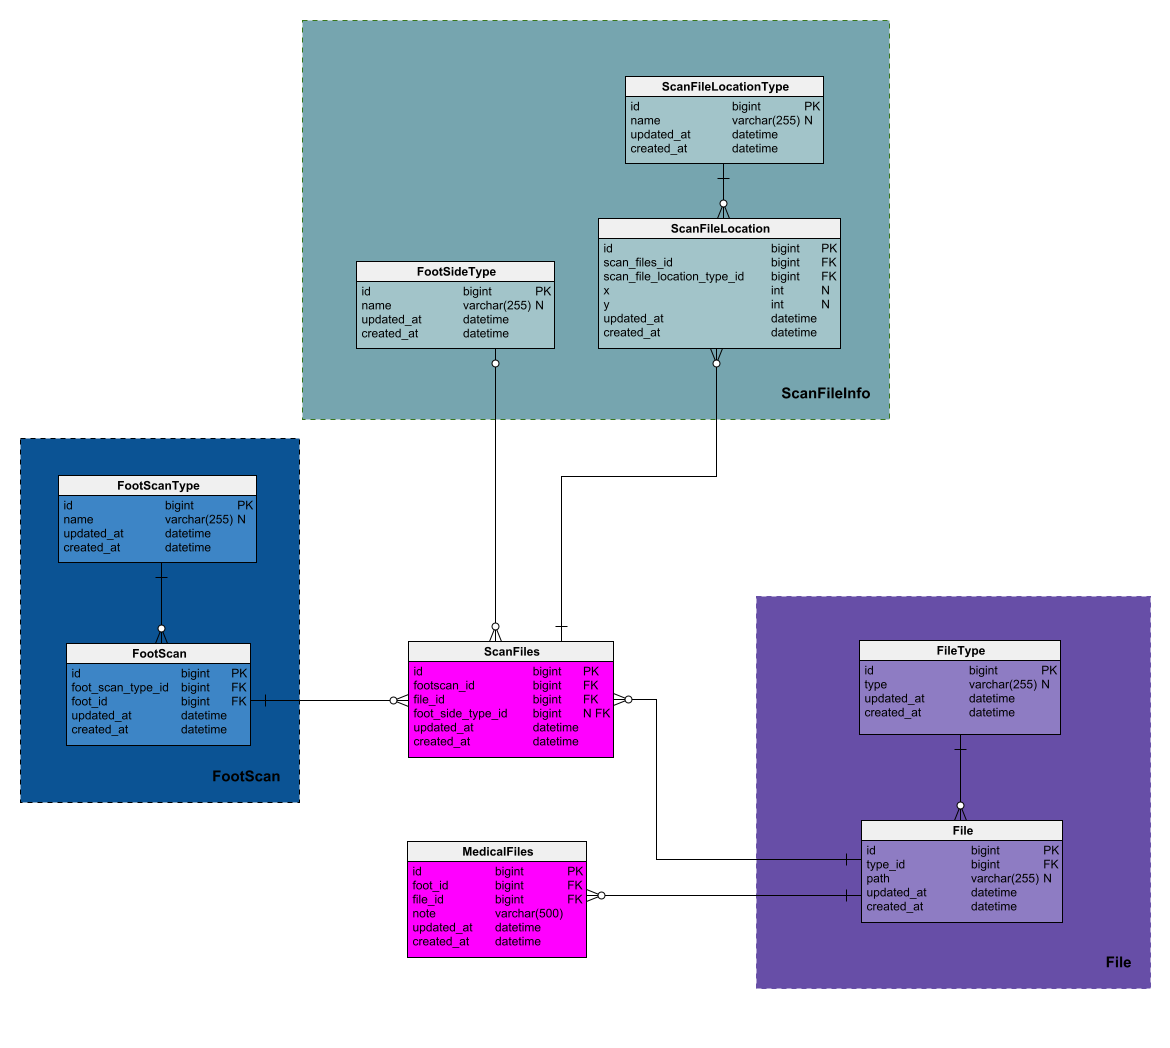
\includegraphics[width=.7\columnwidth]{KaanEksenMSc/figures/DatabaseFiles.png}}
\caption{Database files group}
\label{fig:DatabaseFiles}
\end{figure}

Survey and Training table groups are used for the feedback and healing after deformities are detected. Those tables help the healthcare professionals track the patients' activities. In addition, the DiseaseHistory table group is used to record the previous diseases and surgeries of the patients.

\section{TEST AND EVALUATION} \label{sec:StudyITestAndEvaluation}

In this section, the test and evaluation process of the prototype system, which was explained in detail in the previous sections, will be discussed.

In the first study, the test data were collected through mobile applications without any supervision. Therefore some of the data collected were not usable in the test and evaluation process. In addition, the data was mainly collected on the Yeditepe university students, which is a diverse population, and participants were provided with the how-to-use document.

\begin{table}[htbp]
\begin{center}
\caption{Participant statistics in study I}
\vspace{23pt}
      \begin{tabular}{|c|c|c|c|c|} \hline
          & \textbf{Age} & \textbf{Weight} & \textbf{Height} & \textbf{BMI} \\ \hline
        \textbf{Avarage} & 24.06 & 75.15 & 173.18 & 24.91 \\ \hline
        \textbf{Max} & 48 & 120 & 186 & 37.04 \\ \hline
        \textbf{Min} & 21 & 50 & 160 & 18.14 \\ \hline
    \end{tabular}
\label{tab:StudyIParticipantStatistics}
\end{center}
\end{table}

The prototype was used by 34 participants, where 12 (35.29 percent) of them were female, and the remaining 22 (64,71 percent) were male, with an average age of 24 (see Table \ref{tab:StudyIParticipantStatistics} for details). Data that were provided by participants were stored in an online database which is described in section \ref{sec:StudyIAnalysisAndDesign}. 

\begin{figure}[htbp]
\centering
\fbox{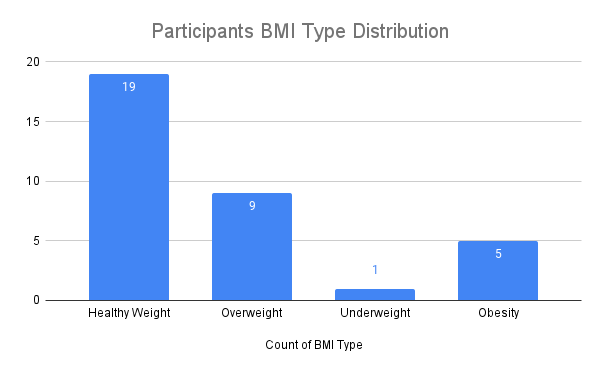
\includegraphics[width=.65\columnwidth]{KaanEksenMSc/figures/StudyIParticipantsBMITypeDistribution.png}}
\caption{Participants BMI type distribution based on CDC in study I}
\label{fig:StudyIParticipantsBMITypeDistribution}
\end{figure}

The average BMI in the population was calculated as 24.9. As seen in Figure \ref{fig:StudyIParticipantsBMITypeDistribution}, at least one person from each BMI category participated in the study. Therefore, this will provide sufficient data for projection.

The data collected from the users included 68 photos, 61 of them were used, but 7 of them were unusable because they were taken incorrectly. In addition, data collection was done in an unsupervised manner which caused seven unusable photos. All the data provided by the participants were shared with a physician through the specialist interface, which is described in sub-section \ref{sec:SpecialistInterface}. The physician went through all the system data and recorded critical points to the system.

\begin{figure}[htbp]
\centering
\fbox{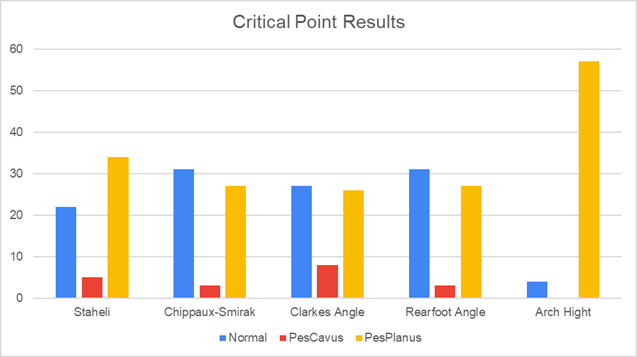
\includegraphics[width=.65\columnwidth]{KaanEksenMSc/figures/StudyICriticalPointResult.png}}
\caption{Critical point results on study I}
\label{fig:StudyICriticalPointResult}
\end{figure}

After the physician results were collected, index calculations were conducted (see Figure \ref{fig:StudyICriticalPointResult}). Even with specialists' critical points, the results vary based on the index type. However, even if the reference points vary, approaching specialists' results will reveal the system's usability. Therefore, the initial study has been investigating the system set critical points, and the specialist set critical point differences.

\begin{figure}[htbp]
\centering
\fbox{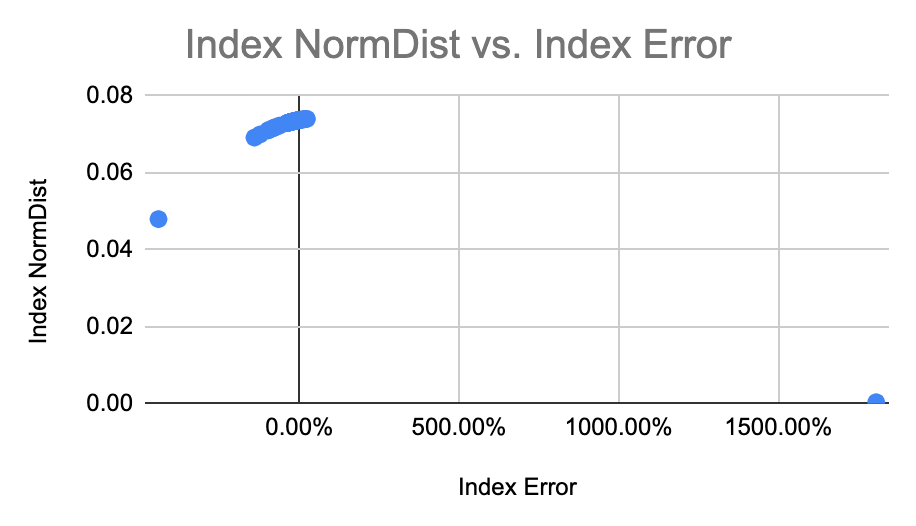
\includegraphics[width=.65\columnwidth]{KaanEksenMSc/figures/StudyIIndexErrorNormalDists.png}}
\caption{Index error normal distribution in study I}
\label{fig:StudyIIndexErrorNormalDists}
\end{figure}

Initial results showed that the findings of the specialist and the system were 91.80 percent matched. Even though these results showed great promise, this comparison was based on the class of the foot. Therefore, a more quantitative approach was necessary to asset the conducted test was accurate. Since automated algorithm critical points are not directly comparable with the specialist critical points (the pre-diagnosis algorithm transforms the images), point intermediate and resulting findings were compared.

Therefore, the system index errors were calculated, and normal distribution was piloted (see Figure \ref{fig:StudyIIndexErrorNormalDists}). The results showed that most of the normal distribution of the index error was within a small error range. On the other hand, it has been observed that there are also outliers with significant error rates. These errors were primarily due to human errors, such as misplaced critical points or photos taken from the wrong angle. 

\begin{figure}[htbp]
\centering
\fbox{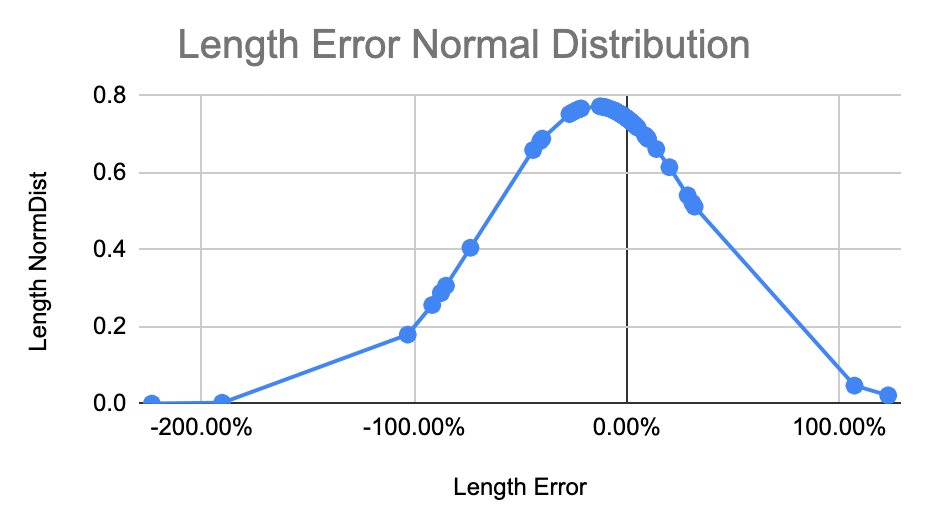
\includegraphics[width=.65\columnwidth]{KaanEksenMSc/figures/StudyILenghtErrorNormalDists.png}}
\caption{Length error normal distribution in study I}
\label{fig:StudyILenghtErrorNormalDists}
\end{figure}

In addition, length error was also calculated to see the effect of the perspective transformation in error calculation (see Figure \ref{fig:StudyILenghtErrorNormalDists}). Even though those results showed similar results to index error, outliers were increased. This error increase was partially due to a perspective transformation of the images.
